\documentclass{article}
\usepackage{amssymb}
\usepackage{graphicx}
\usepackage{caption}
\usepackage{subcaption}
\usepackage{listings}
\usepackage{float} %figure inside minipage
\graphicspath{ {./images/} }
\usepackage[export]{adjustbox}
\usepackage{apacite}
\usepackage{amsmath}

\begin{document}

\section{Zero Cost Defect Control with Hermite-Birkhoff interpolants}
\subsection{Introduction}
In this chapter, we present a zero-cost defect control technique to solve ordinary differential equations (ODE) problems. Typically, Runge-Kutta solvers solve an ODE by providing a discrete solution. They effectively adaptively divide the time domain into steps and return an estimate of the solution at each step. To get a continuous solutions, the user will have to fit an interpolant over the whole region and then sample this interpolant. 

The problem is that there is no guarantee that the interpolant are as accurate as the solution calculated by the solver. Thus if the solver returned a solution that satisfied a tolerance of $10^{-i}$, there are no guarantee that in the middle of the steps, the tolerance is indeed $10^{-i}$. We show using the python Scipy library that even the robust solvers in python that doing an interpolation does not guarantee an accurate solution in Section $\ref{section:end_of_step_innacurate}$ . 

For most scenarios, researchers would usually simply increase the tolerance when there results are not satisfactory,  However, as researchers get tasked to solve more and more complex problems, especially when the ODE problem is part of a much bigger problem like a boundary value problem and others, the need for some sort of error control of the continuous solutions become vital.

There were several methods previously examined for control of the continuous solution and we discuss them in Section $\ref{section:crk_related_work}$ but those methods turn out to be very costly. In this paper we will discuss a zero-cost method to control the error of the continuous solution using Hermite Birkhoff interpolants. We will control the defect along a step, the difference between the actual value of $ft, y)$ and the computed solution's derivative and show how this returns a spline interpolant of the solution over the whole time domain with errors within the tolerance.

We start by discussing the ODE problems we will use to demonstrate our technique in Section $\ref{section:defect_problem_used}$. We then give an overview of the problem with using error control only at the end of the step in Section $\ref{section:end_of_step_innacurate}$. We discuss related work in Section $\ref{section:crk_related_work}$. We give an explanation of the proof of concept solvers that we use in this chapter in Section $\ref{section:basic_runge_kutta}$. 

\subsubsection{Problems used}
\label{section:defect_problem_used}
In this section, we give an explanation of the three problems that we use 

The first problem that we attempt to solve is as follows.
The model is:
\begin{equation}
y'(t, y) = - \frac{y^{3}}{2} 
\end{equation}
The initial condition are y = 1 and the time domain is [0, 10].

The solution to this problem is as shown in Figure $\ref{fig:solution_problem1}$:
\begin{equation}
y(t) = \frac
{1}
{\sqrt{1 + t}}
\end{equation}

The solution looks like:
\begin{figure}[H]
\centering
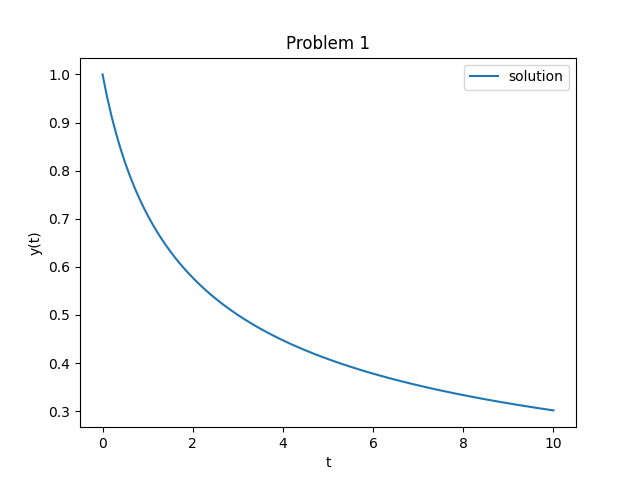
\includegraphics[width=0.7\linewidth]{./figures/solution_problem1}
\caption{Solution to the first ODE problem used in this chapter}
\label{fig:solution_problem1}
\end{figure}

The second problem that we attempt to solve is as follows.
The model is:
\begin{equation}
y'(t, y) = \frac{y(1 - \frac{y}{20})}
{4} 
\end{equation}
The initial condition are y = 1 and the time domain is [0, 10].

The solution to this problem is as follows:
\begin{equation}
y(t) = \frac{20}{1 + 19e^{-\frac{t}{4}}}
\end{equation}

The solution is shown in Figure $\ref{fig:solution_problem2}$:
\begin{figure}[H]
\centering
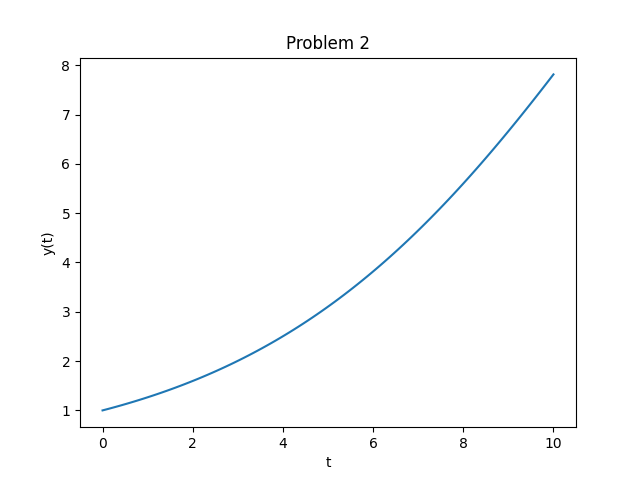
\includegraphics[width=0.7\linewidth]{./figures/solution_problem2}
\caption{Solution to the second ODE problem used in this chapter}
\label{fig:solution_problem2}
\end{figure}

The third problem that we attempt to solve is as follows.
The model is:
\begin{equation}
y'(t, y) = -0.1y - e^{-0.1t}sin(t)
\end{equation}
The initial condition are y = 1 and the time domain is [0, 10].

The solution to this problem is as shown in Figure $\ref{fig:solution_problem3}$:
\begin{equation}
y(t) = e^{-0.1t}cos(t)
\end{equation}

The solution looks like:
\begin{figure}[H]
\centering
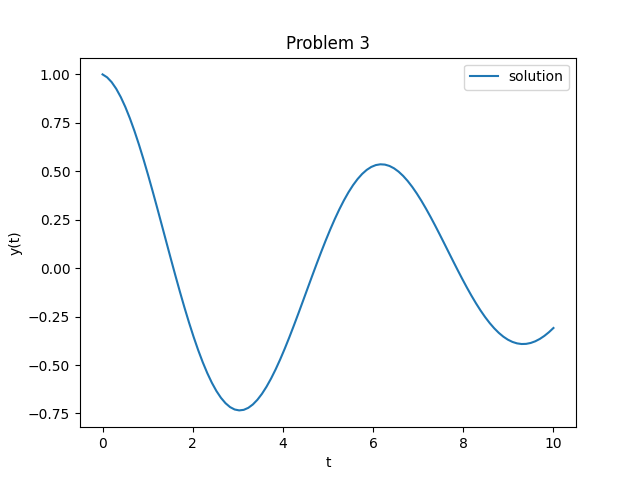
\includegraphics[width=0.7\linewidth]{./figures/solution_problem3}
\caption{Solution to the third ODE problem used in this chapter}
\label{fig:solution_problem3}
\end{figure}

\subsubsection{Lack of Defect Control of end of step solvers}
\label{section:end_of_step_innacurate}
In this section, we talk about how conventional solvers employed in popular packages like the Scipy library solves ODE problems. These libraries will often have the option of using a Runge-Kutta pair solver which works as follows. The pair comes with a low order method and a high order method and will solve the problem by taking a sequence of steps. The solver will take each step with both methods and use the difference between the higher order method and the lower order method to generate an error estimate. If the error estimate is within the user provided tolerance, the solver will accept the step and proceed to the next step. If the error estimate is not within the tolerance, the solver will reduce the step-size and attempt to take the step again. As the error of Runge-Kutta methods depends on the step-size, a smaller step-size will produce a smaller error. The solver will keep reducing the step-size until the user tolerance is satisfied and will then proceed. In an attempt to improve the efficiency, several solvers will also increase the step-size when the tolerance is satisfied by a lot. The solver will then return the sequence of the step produced by the higher order method or the lower method, based on some heuristics.  

The problem with this approach is that the error estimate is produced only at the end of a step and thus the error control is only applied at the end of the step. It is assumed that the solution in the middle of the step is within the user-provided tolerance. However as we will show below, this is sometimes not the case.

The second problem with this approach is that it does not provide a continuous solution and thus, as the user will often ask for output in the middle of steps, the solvers are fitted with an interpolant. For this interpolant to provide a solution within the user provided tolerance, the interpolation error must be less than the error of the data points being fitted. Thus we would ideally use an interpolant at least of order $O(h^{p})$ if the solution is of order $O(h^{p})$. However, for high order methods like a $8^{th}$ order method, it becomes too expensive to fit an $8^{th}$ order interpolant as there are no ways to get enough data points without losing efficiency. These solvers will thus usually compromise and try to fit the highest order interpolant that can be fitted given the amount of data points. 

Finding a continuous solution that fits within the user-provided tolerance is thus a challenge as we are both not guaranteed that the solution in the middle of a step is error-controlled and not guaranteed that interpolation error will not affect our solution. Below is some examples of Runge Butta methods used on the 3 problems above where the tolerance is not controlled.

\begin{figure}[H]
\centering
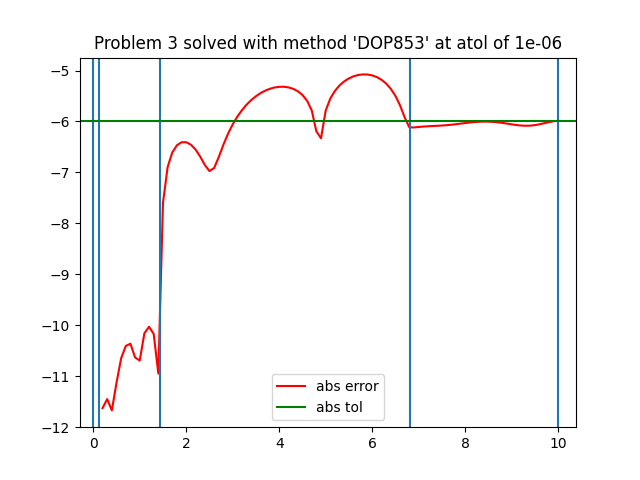
\includegraphics[width=0.7\linewidth]{./figures/no_middle_step_error_control_p3_dop853}
\caption{Scipy `DOP853' on problem 3 at an absolute tolerance of $10^{-6}$ and a relative tolerance of $10^{-6}$}
\label{fig:no_middle_step_error_control_p3_dop853}
\end{figure}

\begin{figure}[H]
\centering
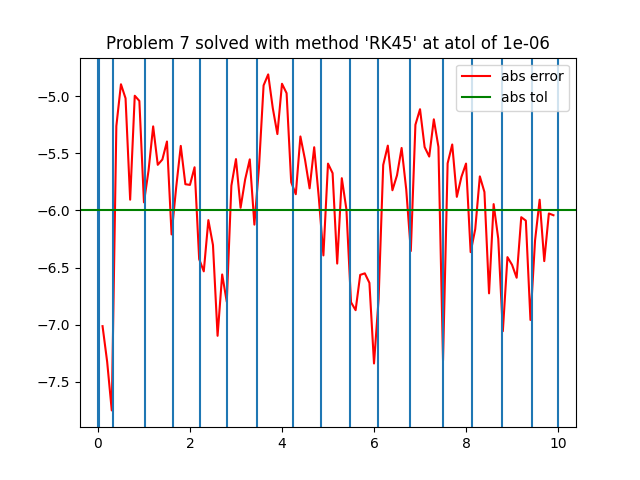
\includegraphics[width=0.7\linewidth]{./figures/no_middle_step_error_control_p7_rk45}
\caption{Scipy `RK45' on problem 7 at an absolute tolerance of $10^{-6}$ and a relative tolerance of $10^{-6}$}
\label{fig:no_middle_step_error_control_p7_rk45}
\end{figure}

Figure $\ref{fig:no_middle_step_error_control_p3_dop853}$ and $\ref{fig:no_middle_step_error_control_p7_rk45}$ shows the errors in the middle of a step of using `DOP853' on problem 3 and `RK45' on problem 7 at an absolute tolerance of $10^{-6}$ and a relative tolerance of $10^{-6}$. They are `classic' error plots in that the solvers were created to behave this way. The only guarantee that the solution is accurate at the end of the step and not in the middle of the step. However we can clearly see that though we asked them to give a solution within a tolerance of $10^{-6}$, the solutions in the middle of the steps reach errors up to one order of magnitude away of that tolerance at $10^{-5}$. 

We now note that whenever a researcher asks for a solution within a tolerance of $10^{-i}$, they expect the solutions from these solvers to be within that tolerance for the whole time domain. However, the decision of not completely satisfying the user provided tolerance was made in the interest of efficiency and the loss of accuracy in the middle of the step was a tradeoff. Modern problems now require that even the solution in the middle of the step is accurate as ODE system solvers are now integral part of bigger software where their results are differentiated, integrated and manipulated in a ways that a continuous solution, especially, a very accurate continuous solution is required. 

In this chapter, we attempt to provide a zero-cost way of controlling the error in the middle of the step and thus throughout the whole time domain. A successful zero-cost accurate interpolant will solve the biggest problem with continuous runge kutta solutions, which is the inefficiency encountered in building these solutions. 

\subsubsection{Defect Control and the cost of traditional Continuous Runge-Kutta method}
\label{section:crk_related_work}
In this section we introduce the `defect' of an ODE solution and explain how the control of the defect guarantees error control and thus why building an interpolant with defect control allows us to get error control of the continuous solution.

In the context of numerical ODEs the defect, denoted by $\delta(t)$,  is the absolute difference between the derivative of the solution computed by a solver, $\bar{f}'(t)$, and the actual derivative of the problem, the user-provided model $f(t, y)$. 

\begin{equation}
\delta(t) = \bar{f}'(t) - f(t, y)
\end{equation}

============
Talk about how the defect controls the error. I think you said something about if the defect is with $10^{p}$, then the error is within $10^{p+1}$. can you confirm?
============

Calculating the defect requires that the solution computed by the solver be differentiable. The idea of defect control is relatively new as differentiable solutions to ODEs are very expensive to calculate. One such attempt is outlined in 8888 reference to Wayne Enright CRK defect control 8888. In this paper, the defect control method that was employed has a number of stages that grows exponentially with the order of the method as shown in Table 888 refer to table below 8888. The method is based on traditional continuous Runge Kutta methods (CRK). In this paper we will produce a defect controlled continuous solution with no additional cost. A typical Runge-Kutta solver will thus be able to take the usual number of stages as other discrete Runge-Kutta method of the same order and still produce an accurate continuous solution.

======================================
Include table order of method versus number of stages.
======================================

Discussion of Enright's work
https://www.cs.toronto.edu/~enright/recentMSc.html

=========
Is there more related work that you want to talk about?
========

Though the defect is defined for the whole step, the concept of the maximum defect within a step is what is more important. The maximum defect within a step is the biggest absolute difference between the derivative of the computed solution at the user provided model within a step. Thus if the maximum defect is within the tolerance, the whole solution within the given step is within the tolerance. The key problem is thus to find the maximum defect within the step. An idea would be to sample the defect at several points and use the maximum value sampled. The problem with this approach is that given a discrete solution, each sampling of the defect requires an additional function evaluation. Thus we cannot make too many sample. The work above solves this problem by defining interpolants that guarantees that the maximum defect is at the same location within a step, halfway through the step. This way only one function evaluation is required to sample the defect. In the approach outlined in this paper, the defect will be guaranteed to be at one of two locations within the step. This way only two samplings must be done to get the maximum defect. Though we make an additional function evaluation, using less stages guarantees that our method is faster especially for higher orders.


\subsubsection{Small explanation of the Runge Kutta methods and the code we have written}
\label{section:basic_runge_kutta}
In this chapter, we will modify simple solvers based on each of 3 Runge-Kutta methods and show that the modification allowed them to produce an accurate continuous solution without having to use any additional stages. In this section, we give an outline of the modifications that were made.

The first Runge-Kutta method upon which we build a defect control solver is the classical $4^{th}$ order Butcher method that uses 4 stages, the second method is a Jim Verner $6^{th}$ order method, taken from his 6(5) pair 8888 need to look for a reference 8888, that uses 9 stages and the last method is an $8^{th}$ order method that uses 13 stages, 8888 Need a reference for that as well 8888. 

The solver that was coded uses a simple step selection logic in that if the maximum defect is greater than $0.8tol$, the solver rejects the step and attempts to retake it again with half the step-size. If the maximum defect is less than $0.2tol$, the solver accepts the step and doubles the step-size for the next step. This is done to prove that the usual efficiency optimisations can be applied here as well. We will elaborate on the initial step-size used by each modification later in the chapter.

We now note that the solver is not optimised. A more thorough analysis of how the solver behaves and thus a more refined step selection algorithm will produce a faster solver in practice. The code in this chapter only serves as a proof of concept for a more elaborate solver. 

\subsection{Multisteps interpolants for zero-cost defect control on a single step Runge Kutta method}
In this section we will show modifications of a solver built on the classical $4^{th}$ order Runge Kutta method that allows for defect control. Its step-selection algorithm is as described in Section $\ref{section:basic_runge_kutta}$. We will fit to the Runge-Kutta method an interpolant of $4^{th}$, $6^{th}$ and $8^{th}$ order respectively and explain the challenges and the gain in efficiency and accuracy of each order separately. We will show how they resulted in error control in the middle of the step and how they are each derived.

We first note that Runge-Kutta methods are very convenient in that they are one step methods. At any point, when taking the next step, the method does not have to take into consideration the size of the previous steps and this is convenient as coders can decide the size of the next step in the most optimal way only based on how the solver is satisfying the tolerance at the current step. 

The first interpolant that we discuss is such single step interpolant. It is the classical Hermite cubic of order 4. We will show how this interpolant can be used to perform defect control and discuss the limitations of this approach. 

We then show how a Hermite-Birkhoff interpolant of $6^th$ order can solve the issues that we faced. We will give an overview of how a $6^th$ order interpolant would be derived and show the results of doing defect control on a this interpolant to solve the 3 problems. 

We will then use a similar approach to derive an $8^{th}$ order Hermite-Birkhoff interpolant and show why the same approach will not work. We then discuss another approach to derive an $8^th$ order interpolant that solvers the issue with the previous one and show the results of using this $8^th$ order interpolant on the three problems.


\subsubsection{rk4 with hb4}
The Hermite cubic spline is an interpolant that has had several applications in various solvers. The basic idea is that we can use the derivative data at the data points and not just the data points themselves to get enough data to fit an interpolant. Given points $(t_i, y_i)$ and $(t_{i + 1}, y_{i + 1})$ with derivatives $f_i$ and $f_{i + 1}$ respectively. The interpolant along $[t_i, t_{i + 1}]$ of size $h_i$ is defined using a parameter $\theta$ as such:

\begin{equation}
u(t_i + \theta*h) = h_{00}(\theta)*y_i +  h_i*h_{10}(\theta)*f_i + h_{01}(\theta)*y_{i + 1} + h_i*h_{11}(\theta)*f_{i + 1} 
\end{equation}
and its derivative:
\begin{equation}
u'(t_i + \theta*h) = h_{00}'(\theta)*y_i/h_i +  h_{10}'(\theta)*f_i + h_{01}'(\theta)*y_{i + 1}/h_i + h_{11}'(\theta)*f_{i + 1} 
\end{equation}

where $\theta$ is based on the value of $t$, that we want to sample in the interval [$t_i$, $t_{i + 1}$] of size $h_i$, as such:
\begin{equation}
\theta = (t - t_i) / h_i
\end{equation}

$h_{00}$, $h_{01}$, $h_{10}$ and $h_{11}$ are each cubics of their own and the interpolant is the cubic formed by summing them all. $h_{00}$, $h_{01}$, $h_{10}$ and $h_{11}$ is defined such that $u(t_i)= y_i$, $u'(t_i) = f_i$, $u(t_{i+1}) = y_{i + 1}$ and $u'(t_{i + 1}) = f_{i + 1}$.

when $\theta$ is 0, $t_i + \theta*h_i$ is $t_i$ and thus only $h_{00}(0)$ should be 1 and all the others cubic should evaluate to 0. Also only $h_{10}'(0)$ should be 1 and all the other cubic's derivatives should evaluate to 0.

when $\theta$ is 1, $t_i + \theta*h_i$ is $t_{i + 1}$ and thus only $h_{01}(1)$ should be 1 and all the other cubics should evaluate to 0. Also only $h_{11}'(1)$ should be 1 and all other cubic's  derivatives should be 0.

Given that each of the cubic has the form $a\theta^3 + b\theta^2 + c\theta + d$ and that for each cubic we know what their evaluations for $\theta$ at 0 and 1 and the evaluations of their derivatives for $\theta$ at 0 and 1. We have 4 equations for each. Thus we can solve the system for each to get the values of a, b, c and d for each cubic.

We know note that the derivative of each cubic can be calculated simply by differentiating the polynomial with respect to $\theta$ and thus the derivative of the interpolant can be found and used for defect control (See The Derivative Above).

We note that we need to divide by $h_i$ because of the the derivative of the cubics are defined with respect to $\theta$ and thus we need to apply the chain rule we $d\theta/dt$.

Thus we can calculate the defect in the middle of the step easily using the derivative of the interpolant and a function evaluation. Additionally as we will show below, the maximum defect occurs consistently either at $x_i + 0.4*h_i$ or at $x_i + 0.8*h_i$ so that we just need to sample twice.

We now note that the interpolant comes at no additional cost. We only need $(x_i, y_i, f_i)$ and $(x_{i + 1}, y_{i + 1}, f_{i + 1})$ to be stored. No additional stages or function evaluation is required for the interpolant itself. It is just maximum defect sampling that will require two additional function evaluations.

For the remainder of this chapter, we will refer to the Hermite cubic interpolant as `HB4'.

\paragraph{Problem 1 results}
Figures $\ref{fig:rk4_with_hb4_p1_global_defect}$, $\ref{fig:rk4_with_hb4_p1_global_error}$ and $\ref{fig:rk4_with_hb4_p1_scaled_defects}$ shows the results of using the modification of RK4 with HB4 on Problem 1. We note that an absolute tolerance of $10^{-6}$ is applied on the maximum defect within the step and this can be shown to occur at $0.2h$ and $0.4h$ along a step of size, h. See Figure $\ref{fig:rk4_with_hb4_p1_scaled_defects}$ to see the scaled defect peeking at these points. We note that we successfully control the defect and thus successfully control the error.

\begin{figure}[H]
\centering
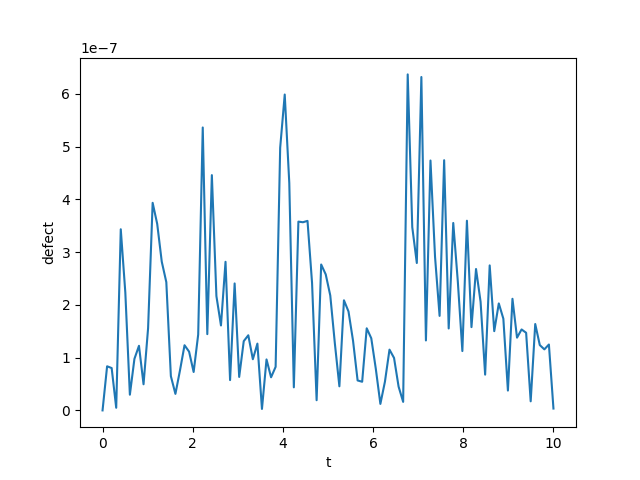
\includegraphics[width=0.7\linewidth]{./figures/rk4_with_hb4_p1_global_defect}
\caption{Global Defect of RK4 with HB4 on problem 1 at an absolute tolerance of $10^{-6}$}
\label{fig:rk4_with_hb4_p1_global_defect}
\end{figure}

\begin{figure}[H]
\centering
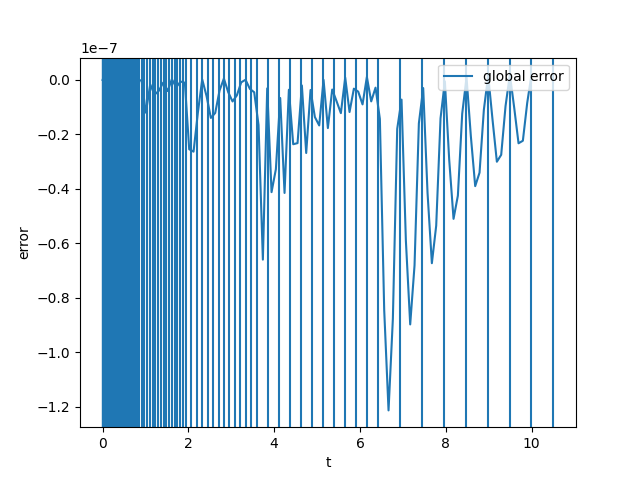
\includegraphics[width=0.7\linewidth]{./figures/rk4_with_hb4_p1_global_error}
\caption{Global Error of RK4 with HB4 on problem 1 at an absolute tolerance of $10^{-6}$}
\label{fig:rk4_with_hb4_p1_global_error}
\end{figure}

\begin{figure}[H]
\centering
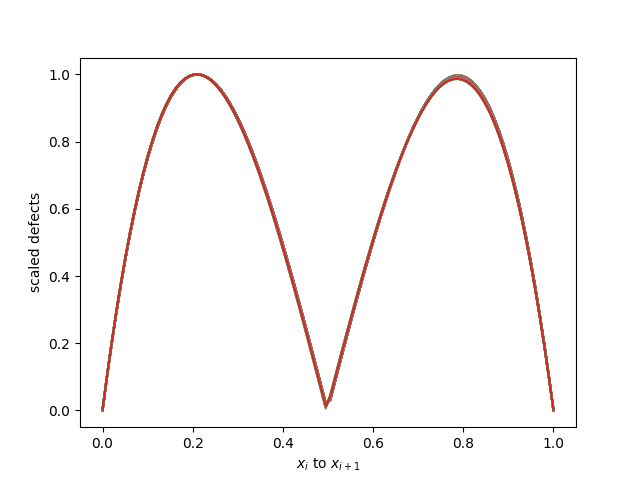
\includegraphics[width=0.7\linewidth]{./figures/rk4_with_hb4_p1_scaled_defects}
\caption{Scaled Defects of RK4 with HB4 on problem 1 at an absolute tolerance of $10^{-6}$}
\label{fig:rk4_with_hb4_p1_scaled_defects}
\end{figure}

\paragraph{Problem 2 results}
Figures $\ref{fig:rk4_with_hb4_p2_global_defect}$, $\ref{fig:rk4_with_hb4_p2_global_error}$ and $\ref{fig:rk4_with_hb4_p2_scaled_defects}$ shows the results of using the modification of RK4 with HB4 on Problem 2. We note that an absolute tolerance of $10^{-6}$ is applied on the maximum defect within the step and this can be shown to occur at $0.2h$ and $0.4h$ along a step of size, h. See Figure $\ref{fig:rk4_with_hb4_p2_scaled_defects}$ to see the scaled defect peeking at these points. We note that we successfully control the defect and thus successfully control the error. For Problem 2, the defect gets noisy on small steps and we do not get two clean peaks. However, we note that we quite consistently get the maximum defects at $0.2h$ and $0.8h$ and thus we only require two samplings.

\begin{figure}[H]
\centering
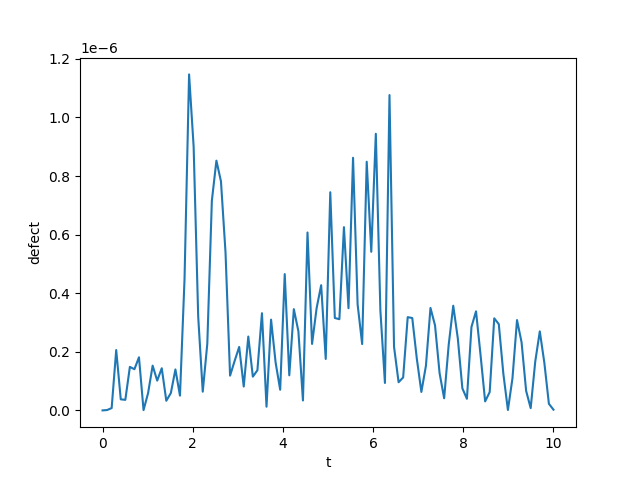
\includegraphics[width=0.7\linewidth]{./figures/rk4_with_hb4_p2_global_defect}
\caption{Global Defect of RK4 with HB4 on problem 2 at an absolute tolerance of $10^{-6}$}
\label{fig:rk4_with_hb4_p2_global_defect}
\end{figure}

\begin{figure}[H]
\centering
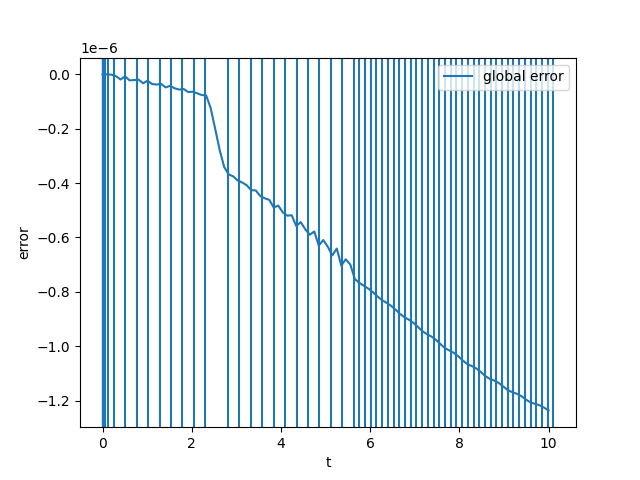
\includegraphics[width=0.7\linewidth]{./figures/rk4_with_hb4_p2_global_error}
\caption{Global Error of RK4 with HB4 on problem 2 at an absolute tolerance of $10^{-6}$}
\label{fig:rk4_with_hb4_p2_global_error}
\end{figure}

\begin{figure}[H]
\centering
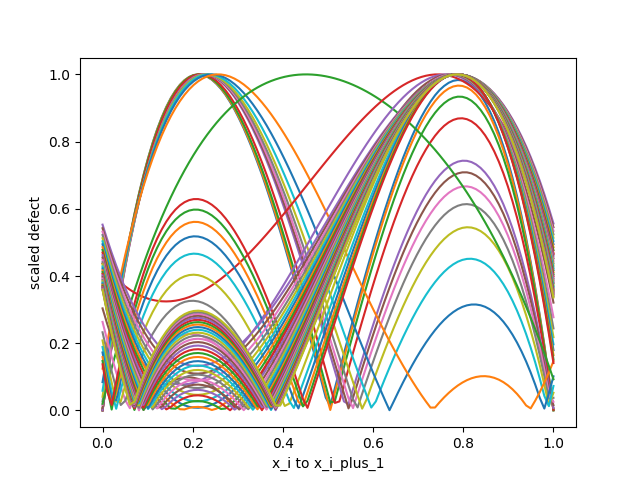
\includegraphics[width=0.7\linewidth]{./figures/rk4_with_hb4_p2_scaled_defects}
\caption{Scaled Defects of RK4 with HB4 on problem 2 at an absolute tolerance of $10^{-6}$}
\label{fig:rk4_with_hb4_p2_scaled_defects}
\end{figure}

\begin{figure}[H]
\centering
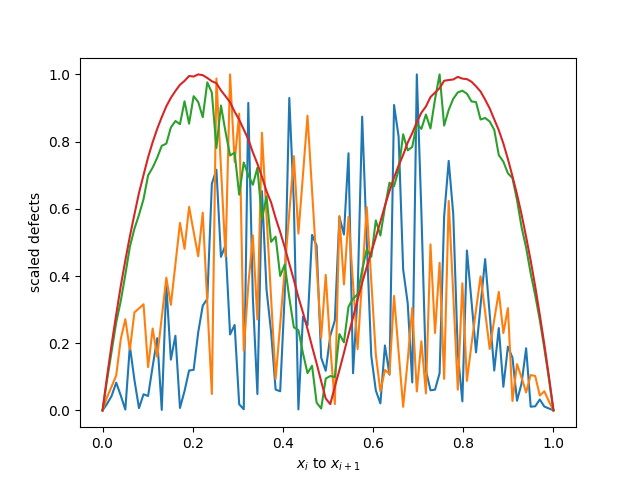
\includegraphics[width=0.7\linewidth]{./figures/rk4_with_hb4_p2_scaled_defects_small_steps}
\caption{Scaled Defects of RK4 with HB4 on small steps on problem 2 at an absolute tolerance of $10^{-6}$}
\label{fig:rk4_with_hb4_p2_scaled_defects_small_steps}
\end{figure}

\paragraph{Problem 3 results}
Figures $\ref{fig:rk4_with_hb4_p3_global_defect}$, $\ref{fig:rk4_with_hb4_p3_global_error}$ and $\ref{fig:rk4_with_hb4_p3_scaled_defects}$ shows the results of using the modification of RK4 with HB4 on Problem 3. We note that an absolute tolerance of $10^{-6}$ is applied on the maximum defect within the step and this can be shown to occur at $0.2h$ and $0.4h$ along a step of size, h. See Figure $\ref{fig:rk4_with_hb4_p3_scaled_defects}$ to see the scaled defect peeking at these points. We note that we successfully control the defect and thus successfully control the error.

\begin{figure}[H]
\centering
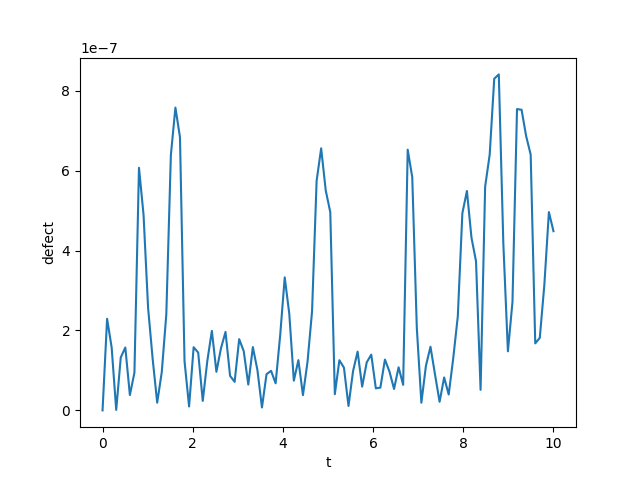
\includegraphics[width=0.7\linewidth]{./figures/rk4_with_hb4_p3_global_defect}
\caption{Global Defect of RK4 with HB4 on problem 3 at an absolute tolerance of $10^{-6}$}
\label{fig:rk4_with_hb4_p3_global_defect}
\end{figure}

\begin{figure}[H]
\centering
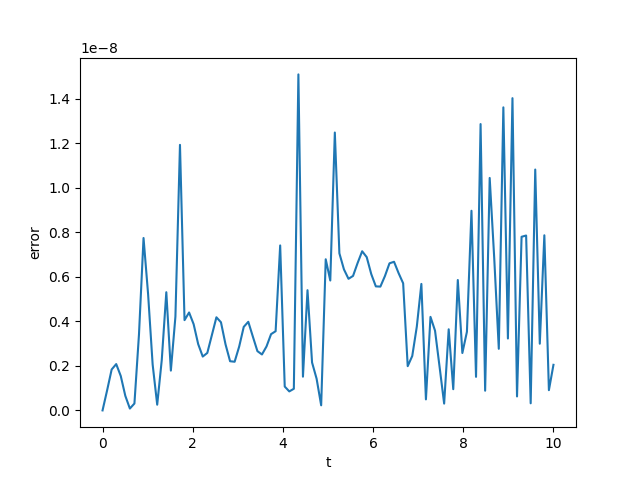
\includegraphics[width=0.7\linewidth]{./figures/rk4_with_hb4_p3_global_error}
\caption{Global Error of RK4 with HB4 on problem 3 at an absolute tolerance of $10^{-6}$}
\label{fig:rk4_with_hb4_p3_global_error}
\end{figure}

\begin{figure}[H]
\centering
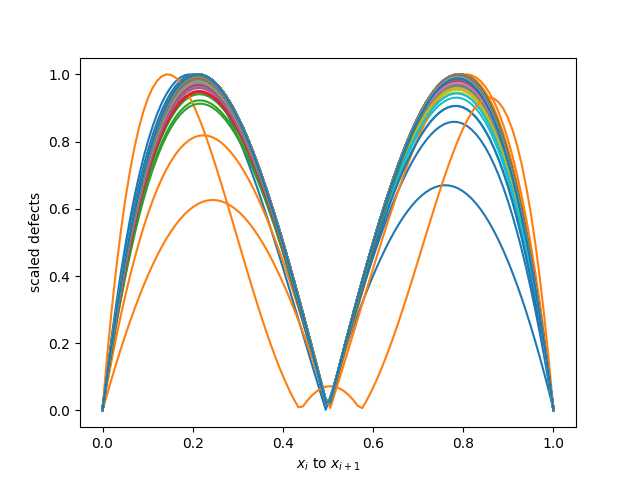
\includegraphics[width=0.7\linewidth]{./figures/rk4_with_hb4_p3_scaled_defects}
\caption{Scaled Defects of RK4 with HB4 on problem 3 at an absolute tolerance of $10^{-6}$}
\label{fig:rk4_with_hb4_p3_scaled_defects}
\end{figure}

\paragraph{efficiency data and discussion of the interpolation error}
We now present the number of steps that were taken by the solver to solve each problem along with the number of successful steps.

\begin{table}[h]
\caption {Number of steps taken by RK4 when modified to do defect control with HB4} \label{tab:rk4_with_hb4_nsteps}
\begin{center}
\begin{tabular}{ c c c } 
Problem & number of successful steps & number of steps \\ 
1       & 84                         & 112 \\ 
2       & 63                         & 109 \\
3       & 238                        & 385 \\
\end{tabular}
\end{center}
\end{table}

We start our discussion by noting that we are not using an efficient step selection algorithm. Still such a high number of steps in all 3 cases is alarming and easy to explain.

The Hermite cubic, HB4, produces an interpolant of $4^{th}$ order. However, to perform defect control we need to calculate the derivative of this interpolant. With this scheme of using the derivative to create the interpolant, the order of the derivative is 3 and we lose one order for each subsequent derivative. The numerical solution is of order 4 as we are using the classical rk4 and thus the derivative of the interpolant is less accurate than the ODE solution. We need a way to get an interpolant whose derivative is at least of order 4 so that the interpolation error does not interfere with our results.

To do that, in the next section, we will introduce a new interpolation scheme called the Hermite-Birkhoff interpolant which is of $6^{th}$ order and will thus have a derivative of order 5.

\subsubsection{rk4 with HB6}
We will use the idea from the Hermite cubic to create a Hermite-Birkhoff interpolant of order 6. We first start by noting that this interpolant is a multistep interpolant as it depends on the previous step.

Suppose that the steps taken by a solver to go from $t_i$ to $t_{i + 1}$ is of size $h$. We can define the size of the step from $t_{i - 1}$ to $t_i$ by using a weight $\alpha$ such that the size of the step from $t_{i - 1}$ to $t_i$ is $\alpha$h. Then given the solution values and the derivative values at all the three points, i.e $(t_{i-1}, y_{i - 1}, f_{i - 1})$, $(t_i, y_i, f_i)$ and $(t_{i + 1}, y_{i + 1}, f_{i + 1})$, we can fit a two step interpolant of order 6 by using a quintic defined as such:
\begin{equation}
\begin{split}
u(t_i + \theta*h) = d_{0}(\theta)*y_{i-1} +  h_i*d_{1}(\theta)*f_{i-1} \\
+ d_{2}(\theta)*y_i     +  h_i*d_{3}(\theta)*f_i \\
+ d_{4}(\theta)*y_{i + 1} + h_i*d_{5}(\theta)*f_{i + 1} \\
\end{split}
\end{equation}
and its derivative is
\begin{equation}
\begin{split}
u'(t_i + \theta*h) = d_{0}'(\theta)*y_{i-1}/h_i +  d_{1}'(\theta)*f_{i-1} \\
+ d_{2}'(\theta)*y_i/h_i     +  d_{3}'(\theta)*f_i \\
+ d_{4}'(\theta)*y_{i + 1}/h_i + d_{5}'(\theta)*f_{i + 1} \\
\end{split}
\end{equation}

where $\theta$ is based on the value of $t$, that we want to sample in the interval [$t_i$, $t_{i + 1}$] of size $h_i$, as such:
\begin{equation}
\theta = (t - t_i) / h_i
\end{equation}

This time $\theta$ is allowed to vary between -$\alpha$ and 1 such that $t_i + \theta$h is at $t_{i - 1}$ when $\theta$ is $-\alpha$, at $t_i$ when $\theta$ is at 0 and $t_{i + 1}$ when theta is 1. Also $d_0$, $d_1$, $d_2$, $d_3$, $d_4$, and $d_5$ are all quintic polynomials and will each have 6 conditions from which we can build a system to find their coefficients in terms of $\alpha$.

Each is a quintic of the form $a\theta^5 + b\theta^4 + c\theta^3 + d\theta^2 + e\theta + f$ where the six coefficients for each can be found in terms of $\alpha$ by solving a linear system of 6 equations in terms of $\alpha$. First at $\theta = -\alpha$, only $d_0(\theta)$ evaluates to 1 and all the other quintic polynomials evaluate to 0 as $u(t_i - \alpha h) = u(t_{i - 1}) = y_{i - 1}$. Also at this theta, only the derivative of $d_1$ evaluates to 1 and all the other quintic polynomials' derivatives evaluate to 0 as $u'(t_i - \alpha h) = u'(t_{i - 1}) = f_{i - 1}$. When $\theta$ is at 0, only $d_2(\theta)$ evaluates to 1 and all the other polynomials evaluate to 0 as $u(t_i - 0*h) = u(t_i) = y_i$. Also at this theta, only the derivative of $d_3$ evaluates to 1 and all the other quintic polynomials' derivatives evaluate to 0 as $u'(t_i - 0*h) = u'(t_i) = f_i$. When $\theta$ is at 1, only $d_4(\theta)$ evaluates to 1 and all the other polynomials evaluate to 0 as $u(t_i + 1*h) = u(t_{i+1}) = y_{i+1}$. Also at this theta, only the derivative of $d_5$ evaluates to 1 and all the other quintic polynomials' derivatives evaluate to 0 as $u'(t_i - 1*h) = u'(t_{i+1}) = f_{i+1}$. With these size conditions, we can get six equations for each quintic in terms of $\alpha$ and using a symbolic management package, we can solve all of these to find the six quintic polynomials.

We again note that as the solver is stepping through a problem, these interpolants are created for free. We just need to store the 3 data points $(t_{i-1}, y_{i - 1}, f_{i - 1})$, $(t_i, y_i, f_i)$ and $(t_{i + 1}, y_{i + 1}, f_{i + 1})$ and run the equation for $u(t + \theta h)$. We will also see that the defects peak at two positions along a step and thus, we can find the maximum defect by only sampling twice. This technique essentially provides, zero-cost defect control and result in an accurate continuous solution.

The interpolant defined as above will now be referred to as hb6 for the remainder of this chapter. We note that it is of order 6 and its derivative is of order 5 and any subsequent higher derivative will be of one less order. The derivative can can again be found by differentiating each quintic seperately with respect to $\theta$ and then dividing by $1/h_i$, to use the chain rule, to get the derivative of the final polynomial.

We now note that on rk4 as the data points are only accurate to $4^{th}$ order, we would want the derivative of the interpolant to be of order 4 or higher so that interpolation error is negligible. This scheme satisfies this condition and we will see below how this allows us to take less steps.

\paragraph{Problem 1 results}
Figures $\ref{fig:rk4_with_hb6_p1_global_defect}$, $\ref{fig:rk4_with_hb6_p1_global_error}$ and $\ref{fig:rk4_with_hb6_p1_scaled_defects}$ shows the results of using the modification of RK4 with HB6 on Problem 1. We note that an absolute tolerance of $10^{-6}$ is applied on the maximum defect within the step and this can be shown to occur at $0.4h$ and $0.8h$ along a step of size, h. See Figure $\ref{fig:rk4_with_hb6_p1_scaled_defects}$ to see the scaled defect peaking at these points. We note that we successfully control the defect and thus successfully control the error.

\begin{figure}[H]
\centering
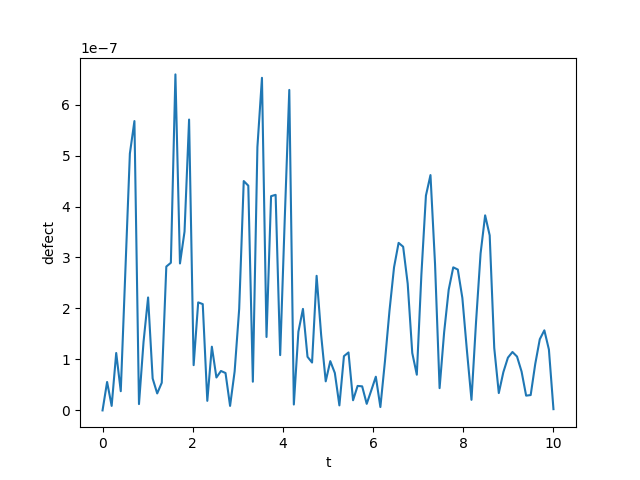
\includegraphics[width=0.7\linewidth]{./figures/rk4_with_hb6_p1_global_defect}
\caption{Global Defect of RK4 with HB6 on problem 1 at an absolute tolerance of $10^{-6}$}
\label{fig:rk4_with_hb6_p1_global_defect}
\end{figure}

\begin{figure}[H]
\centering
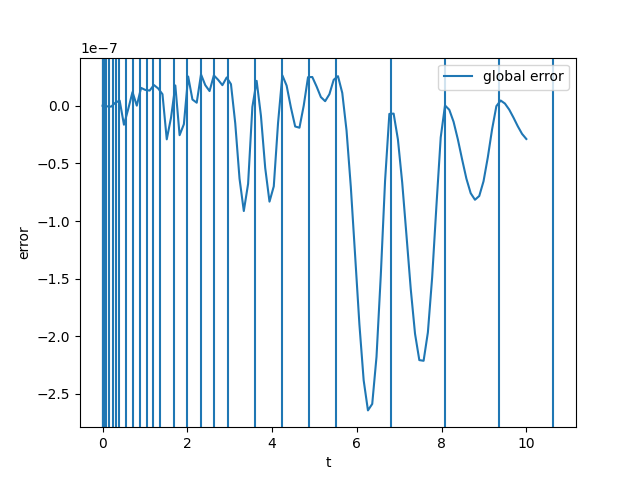
\includegraphics[width=0.7\linewidth]{./figures/rk4_with_hb6_p1_global_error}
\caption{Global Error of RK4 with HB6 on problem 1 at an absolute tolerance of $10^{-6}$}
\label{fig:rk4_with_hb6_p1_global_error}
\end{figure}

\begin{figure}[H]
\centering
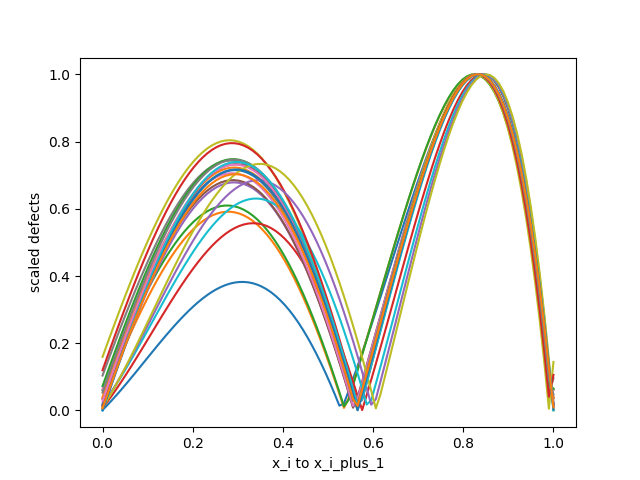
\includegraphics[width=0.7\linewidth]{./figures/rk4_with_hb6_p1_scaled_defects}
\caption{Scaled Defects of RK4 with HB6 on problem 1 at an absolute tolerance of $10^{-6}$}
\label{fig:rk4_with_hb6_p1_scaled_defects}
\end{figure}

\paragraph{Problem 2 results}
Figures $\ref{fig:rk4_with_hb6_p2_global_defect}$, $\ref{fig:rk4_with_hb6_p2_global_error}$ and $\ref{fig:rk4_with_hb6_p2_scaled_defects}$ shows the results of using the modification of RK4 with HB6 on Problem 2. We note that an absolute tolerance of $10^{-6}$ is applied on the maximum defect within the step and this can be shown to occur at $0.4h$ and $0.8h$ along a step of size, h. See Figure $\ref{fig:rk4_with_hb6_p2_scaled_defects}$ to see the scaled defect peeking at these points. We note that we successfully control the defect and thus successfully control the error. For Problem 2, the defect gets noisy on small steps and we do not get two clean peaks. However, we note that we quite consistently get the maximum defects at $0.2h$ and $0.8h$ and thus we only require two samplings.

\begin{figure}[H]
\centering
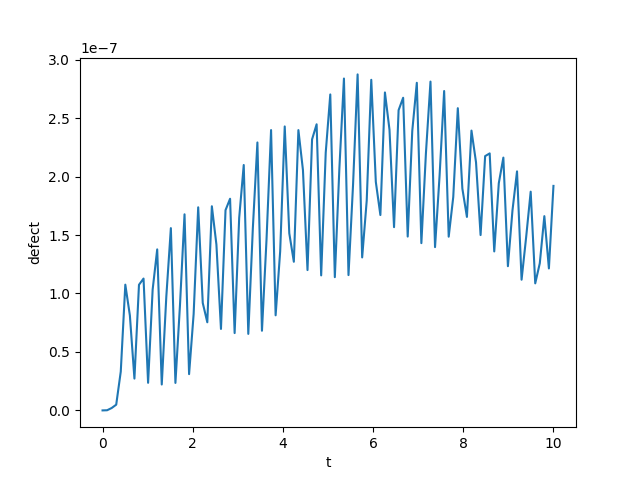
\includegraphics[width=0.7\linewidth]{./figures/rk4_with_hb6_p2_global_defect}
\caption{Global Defect of RK4 with HB6 on problem 2 at an absolute tolerance of $10^{-6}$}
\label{fig:rk4_with_hb6_p2_global_defect}
\end{figure}

\begin{figure}[H]
\centering
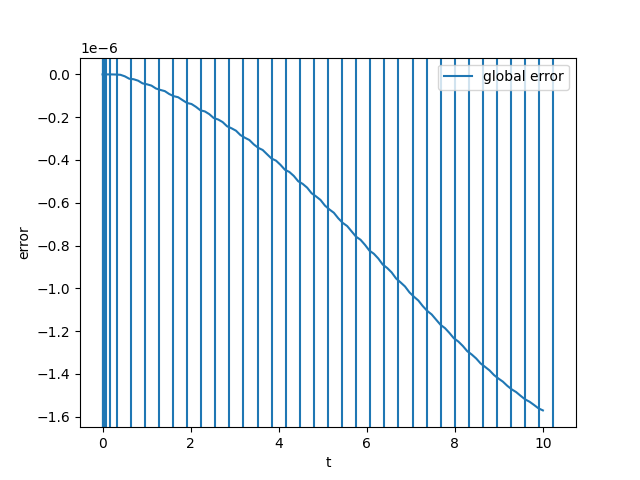
\includegraphics[width=0.7\linewidth]{./figures/rk4_with_hb6_p2_global_error}
\caption{Global Error of RK4 with HB6 on problem 2 at an absolute tolerance of $10^{-6}$}
\label{fig:rk4_with_hb6_p2_global_error}
\end{figure}

\begin{figure}[H]
\centering
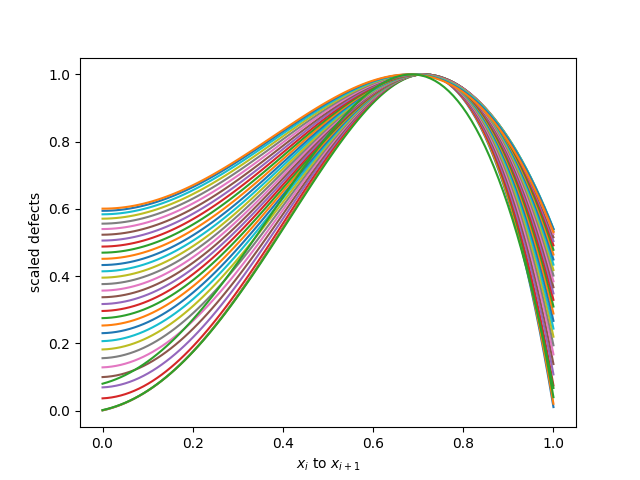
\includegraphics[width=0.7\linewidth]{./figures/rk4_with_hb6_p2_scaled_defects}
\caption{Scaled Defects of RK4 with HB6 on problem 2 at an absolute tolerance of $10^{-6}$}
\label{fig:rk4_with_hb6_p2_scaled_defects}
\end{figure}

\begin{figure}[H]
\centering
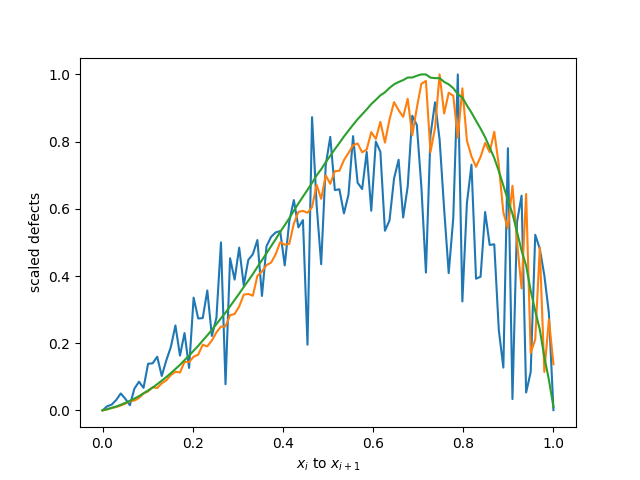
\includegraphics[width=0.7\linewidth]{./figures/rk4_with_hb6_p2_scaled_defects_small_steps}
\caption{Scaled Defects of RK4 with HB6 on small steps on problem 2 at an absolute tolerance of $10^{-6}$}
\label{fig:rk4_with_hb6_p2_scaled_defects_small_steps}
\end{figure}

\paragraph{Problem 3 results}
Figures $\ref{fig:rk4_with_hb6_p3_global_defect}$, $\ref{fig:rk4_with_hb6_p3_global_error}$ and $\ref{fig:rk4_with_hb6_p3_scaled_defects}$ shows the results of using the modification of RK4 with HB6 on Problem 3. 
======================== Note as clear
We note that an absolute tolerance of $10^{-6}$ is applied on the maximum defect within the step and this can be shown to occur at $0.8h$ along a step of size, h. See Figure $\ref{fig:rk4_with_hb6_p3_scaled_defects}$ to see the scaled defect peeking at these points. We note that we successfully control the defect and thus successfully control the error.
================================

\begin{figure}[H]
\centering
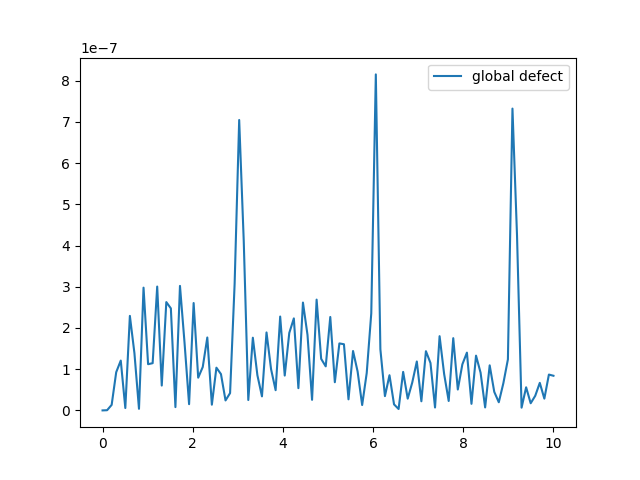
\includegraphics[width=0.7\linewidth]{./figures/rk4_with_hb6_p3_global_defect}
\caption{Global Defect of RK4 with HB6 on problem 3 at an absolute tolerance of $10^{-6}$}
\label{fig:rk4_with_hb6_p3_global_defect}
\end{figure}

\begin{figure}[H]
\centering
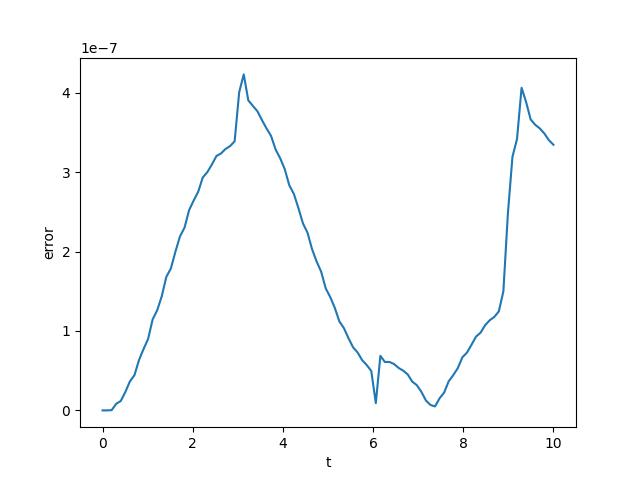
\includegraphics[width=0.7\linewidth]{./figures/rk4_with_hb6_p3_global_error}
\caption{Global Error of RK4 with HB6 on problem 3 at an absolute tolerance of $10^{-6}$}
\label{fig:rk4_with_hb6_p3_global_error}
\end{figure}

\begin{figure}[H]
\centering
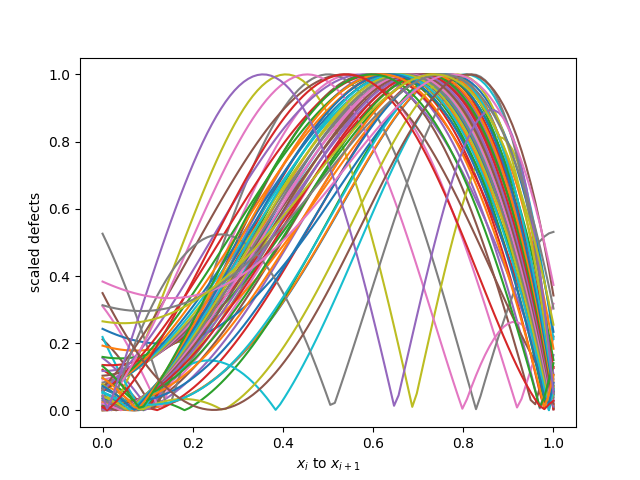
\includegraphics[width=0.7\linewidth]{./figures/rk4_with_hb6_p3_scaled_defects}
\caption{Scaled Defects of RK4 with HB6 on problem 3 at an absolute tolerance of $10^{-6}$}
\label{fig:rk4_with_hb6_p3_scaled_defects}
\end{figure}

We note that the defects are not as clean they were in the case with HB4. There are two peaks most of the time at around $0.4h$ and $0.8h$ but as was the case in the third problem, the peak sometimes comes at $0.6h$. However, we can see that the defect is still being controlled and thus that the error is still being controlled. We will also see that it is twice as fast as it uses around half the number of steps as HB4.

\begin{table}[h]
\caption {Number of steps taken by RK4 when modified to do defect control with HB6 vs when modified with HB4} \label{tab:rk4_with_hb6_nsteps}
\begin{center}
\begin{tabular}{ c c c c c } 
Problem & n. successful steps HB4 & n. successful steps HB6 & nsteps HB4  & nsteps HB6 \\ 
1       & 84                      &        26               & 112         & 31\\ 
2       & 63                      &        36               & 109         & 66\\
3       & 238                     &        63               & 385         & 101\\
\end{tabular}
\end{center}
\end{table}

Table $\ref{tab:rk4_with_hb6_nsteps}$ shows how the number of steps more than halves when we use hb6 as opposed to hb4. This is entirely because the interpolation error is less than the actual ODE error especially for the derivative.

\paragraph{problems with alpha}
The problem with this scheme is that the interpolant is multistep while Runge-Kutta methods are one step. The Hermite Birkhoff interpolant, HB6, is based on two steps and the parameter $\alpha$ defines how big the previous step is compared to the actual step. The error term in Hermite-Birkhoff interpolants is minimised when the size of the two steps are the same size. The error term is proporitional to $(t + alpha)^2t^2(t + 1)^2$. Slight deviation of $\alpha$ from 1 reduces the accuracy of the solvers.

In Figure $\ref{fig:hb6_alpha_v_shape}$, we perform a simple experiment to show how this scheme depends on the value of $\alpha$. We place 3 data points along the t-axis such that their distance apart are $\alpha$ h and h for several values of $\alpha$ and we vary h from 1 to $10^{-7}$, we then report on the order of the maximum defect at each h for these values.

\begin{figure}[H]
\centering
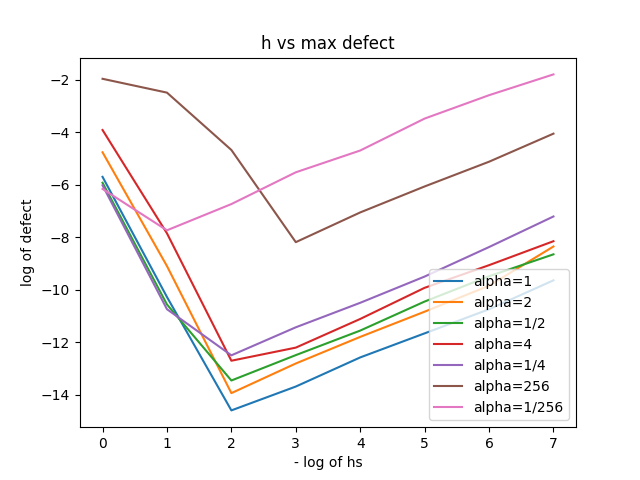
\includegraphics[width=0.7\linewidth]{./figures/hb6_alpha_v_shape}
\caption{HB6 maximum order of accuracy based on different values of alpha}
\label{fig:hb6_alpha_v_shape}
\end{figure}

Figure $\ref{fig:hb6_alpha_v_shape}$ show that at $\alpha$ = 2 and $\frac{1}{2}$, the errors can still reach the orders of magnitude than when $\alpha$ is at 1. However, the orders of magnitude of the error is completely different when $\alpha$ deviates more from 1. We can see that at 256 and $\frac{1}{256}$, we cannot get high accuracy. We will also discuss the V-shape of the graph prompting that there is an optimal h value. (See Section $\ref{section:v_shaped_graph}$).

We note that in solving the 3 problems above, $\alpha$ very rarely was bigger than 4 or smaller than $\frac{1}{4}$ and thus, we can be satisfied with this scheme. We present a solution to the $\alpha$ problem in Section $\ref{section:keeping_alpha_at_1}$.

One more idea would be to use an even higher order interpolant so as to reduce the interpolation error more. We note that with the Hermite-Birkhoff scheme there is no additional cost to get use higher order interpolants. In the next section, we discuss an $8^{th}$ order interpolant and show how to solve the problems of deriving such an interpolant.

\subsubsection{rk4 with HB8}
\paragraph{Derivation of HB8}
In this section, we discuss a derivation of an $8^{th}$ order interpolant. To derive an 8 order method, we need 4 data points and thus build it over 3 steps. We need the data points to be $(t_i, y_i, f_i)$ as well as the two previous steps $(t_{i-1}, y_{i-1}, f_{i-1})$ and $(t_{i-2}, y_{i-2}, f_{i-2})$ and the next step, $(t_{i+1}, y_{i+1}, f_{i+1})$. We present two schemes: 
\begin{itemize}
\item The first scheme when the parameters $\alpha$ and $\beta$ is applied to the previous two steps, so the three steps are of the size $\beta h$, $\alpha h$ and $h$ respectively. Thus the scheme derives the step-size based on the last step. 

\item The second scheme when the parameters $\alpha$ and $\beta$ is applied $\alpha$ on the next step and $\beta$ on the previous step and the middle step being the base size. Thus the sizes for the steps are $\alpha h$, $h$ and then $\beta h$. 

\end{itemize}


\paragraph{First Scheme}
In the first scheme, the step sizes are $\beta h$, $\alpha h$ and $h$ respectively. The interpolant defined on $(t_{i-2}, y_{i-2}, f_{i-2})$, $(t_{i-1}, y_{i-1}, f_{i-1})$, $(t_i, y_i, f_i)$ and $(t_{i + 1}, y_{i + 1}, f_{i + 1})$ are defined as such:

\begin{equation}
\begin{split}
u(t_i + \theta*h) = d_{0}(\theta)*y_{i-2} +  h_i*d_{1}(\theta)*f_{i-2} \\
+ d_{2}(\theta)*y_{i-1}     +  h_i*d_{3}(\theta)*f_{i-1} \\
+ d_{4}(\theta)*y_i     +  h_i*d_{5}(\theta)*f_i \\
+ d_{6}(\theta)*y_{i + 1} + h_i*d_{7}(\theta)*f_{i + 1} \\
\end{split}
\end{equation}
and the derivative is:
\begin{equation}
\begin{split}
u'(t_i + \theta*h) = d_{0}'(\theta)*y_{i-2}/h_i +  d_{1}'(\theta)*f_{i-2} \\
+ d_{2}'(\theta)*y_{i-1}/h_i   +  d_{3}'(\theta)*f_{i-1} \\
+ d_{4}'(\theta)*y_i/h_i       +  d_{5}'(\theta)*f_i \\
+ d_{6}'(\theta)*y_{i + 1}/h_i +  d_{7}'(\theta)*f_{i + 1} \\
\end{split}
\end{equation}
where $\theta$ is based on the value of $t$, that we want to sample in the interval [$t_i$, $t_{i + 1}$] of size $h_i$, as such:
\begin{equation}
\theta = (t - t_i) / h_i
\end{equation}

This time $\theta$ is allowed to vary between $-\alpha-\beta$ and 1 such that $t_i + \theta$h is at $t_{i-2}$ when $\theta$ is $-\alpha-\beta$, at $t_{i-1}$ when $\theta$ is $-\alpha$, at $t_i$ when $\theta$ is at 0 and $t_{i + 1}$ when theta is 1. Also $d_0$, $d_1$, $d_2$, $d_3$, $d_4$, $d_5$, $d_6$ and $d_7$ are all septic polynomials and will each have 8 conditions from which we can build a system to find their coefficients in terms of $\alpha$ and $\beta$.

Each is a septic of the form $a\theta^7 + b\theta^6 + c\theta^5 + d\theta^4 + e\theta^3 + f\theta^2 + g\theta + h$ where the eight coefficients for each can be found in terms of $\alpha$ and $\beta$ by solving a linear system of 8 equations in terms of $\alpha$ and $\beta$. First at $\theta = -\alpha-\beta$, only $d_0(\theta)$ evaluates to 1 and all the other septic polynomials evaluate to 0 as $u(t_i - (\alpha+\beta) h) = u(t_{i - 2}) = y_{i - 2}$. Also at this $\theta$, only the derivative of $d_1$ evaluates to 1 and all the other septic polynomials' derivatives evaluate to 0 as $u'(t_i - (\alpha+\beta) h) = u'(t_{i - 2}) = f_{i - 2}$. When $\theta = -\alpha$, only $d_2(\theta)$ evaluates to 1 and all the other septic polynomials evaluate to 0 as $u(t_i - \alpha h) = u(t_{i - 1}) = y_{i - 1}$. Also at this $\theta$, only the derivative of $d_3$ evaluates to 1 and all the other septic polynomials' derivatives evaluate to 0 as $u'(t_i - \alpha h) = u'(t_{i - 1}) = f_{i - 1}$. When $\theta$ is at 0, only $d_4(\theta)$ evaluates to 1 and all the other polynomials evaluate to 0 as $u(t_i - 0*h) = u(t_i) = y_i$. Also at this theta, only the derivative of $d_5$ evaluates to 1 and all the other septic polynomials' derivatives evaluate to 0 as $u'(t_i - 0*h) = u'(t_i) = f_i$. When $\theta$ is at 1, only $d_6(\theta)$ evaluates to 1 and all the other polynomials evaluate to 0 as $u(t_i + 1*h) = u(t_{i+1}) = y_{i+1}$. Also at this theta, only the derivative of $d_7$ evaluates to 1 and all the other septic polynomials' derivatives evaluate to 0 as $u'(t_i - 1*h) = u'(t_{i+1}) = f_{i+1}$. With these eight conditions, we can get eight equations for each septic in terms of $\alpha$ and $\beta$ and using a symbolic management package, we can solve all of these to find the eight septic polynomials.

We again note that as the solver is stepping through a problem, these interpolants are created for free. We just need to store the 4 data points $(t_{i-1}, y_{i - 1}, f_{i - 1})$, $(t_{i-1}, y_{i - 1}, f_{i - 1})$, $(t_i, y_i, f_i)$ and $(t_{i + 1}, y_{i + 1}, f_{i + 1})$ and run the equation for $u(t + \theta h)$.

The interpolant defined as above will now be referred to as hb8 for the remainder of this chapter. We note that it is of order 8 and its derivative is of order 7 and any subsequent higher derivative will be of one less order. The derivative can can again be found by differentiating each septic seperately with respect to $\theta$ and then dividing by $1/h_i$, to use the chain rule, to get the derivative of the final polynomial.

These scheme has a serious problem. The maximum order in the accuracy is very sensitive to a slight change in $\alpha$ and/or $\beta$. This is beecause the error term is now approximately proportional to $(t + alpha + beta)^2(t+alpha)^2(t)^2(t+1)^2$. We note that the first term depends on both $alpha + beta$ and thus very small deviations in these will result to a very low maximum accuracy. 

In Figure $\ref{fig:hb8_first_scheme_alpha_beta_test}$, we perform a simple experiment to show how this scheme is flawed. We place 4 data points along the t-axis such that their distance apart are $\beta h$, $\alpha h$ and $h$ for several values of $\alpha$ and $\beta$ and we vary h from 1 to $10^{-10}$, we then report on the order of the maximum defect at each h for these values.

\begin{figure}[H]
\centering
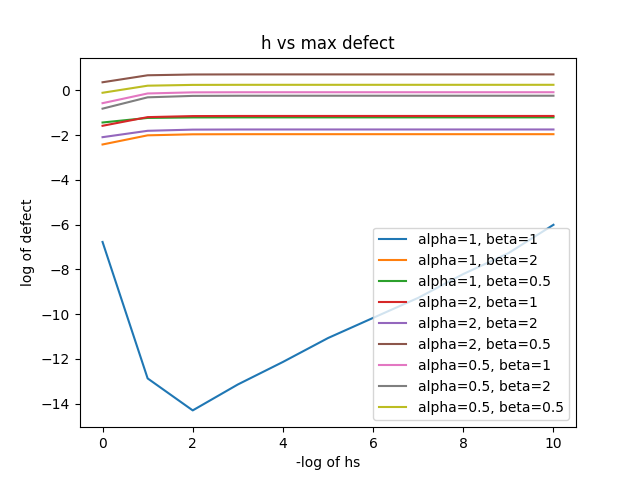
\includegraphics[width=0.7\linewidth]{./figures/hb8_first_scheme_alpha_beta_test}
\caption{HB8 First Scheme - maximum order of accuracy based on different values of alpha and beta}
\label{fig:hb8_first_scheme_alpha_beta_test}
\end{figure}

From Figure $\ref{fig:hb8_first_scheme_alpha_beta_test}$, we can see how this scheme is useless. It only works if both $\alpha$ and $\beta$ are at 1 and even small deviations from 1 of either or both of the weights make the maximum order of accuracy be too small. More importantly, we can never halve the step with this method as if either $\alpha$ or $\beta$ is 2, the solver cannot even get accurate to one order of magnitude. We will know present a better scheme that is more stable to changes in $\alpha$ and $\beta$.

\paragraph{Second Scheme}
In this second scheme, we create a Hermite-Birkhoff interpolant of $8^{th}$ order by picking different locations for the weights of $h$. We still use a 3 step interpolant with 4 data points as the two previous steps $(t_{i-1}, y_{i-1}, f_{i-1})$ and $(t_{i-2}, y_{i-2}, f_{i-2})$ and the next step, $(t_{i+1}, y_{i+1}, f_{i+1})$ but now the distance between the points are $\alpha h$, $h$ and then $\beta h$. The size of the middle step is the base step-size. This way the error term is approximately proportional to $(t- (1+\beta))^2(t+1)^2t^2(t+\beta)^2$. We avoid the $(t-(\alpha+\beta))^2$. We will show that this scheme is more resilient to changes in $\alpha$ and $\beta$.

Its derivation is very similar to the first scheme. The equation for the interpolant is:
\begin{equation}
\begin{split}
u(t_i + \theta*h) = d_{0}(\theta)*y_{i-2} +  h_i*d_{1}(\theta)*f_{i-2} \\
+ d_{2}(\theta)*y_{i-1}     +  h_i*d_{3}(\theta)*f_{i-1} \\
+ d_{4}(\theta)*y_i     +  h_i*d_{5}(\theta)*f_i \\
+ d_{6}(\theta)*y_{i + 1} + h_i*d_{7}(\theta)*f_{i + 1} \\
\end{split}
\end{equation}
and its derivative is:
\begin{equation}
\begin{split}
u'(t_i + \theta*h) = d_{0}'(\theta)*y_{i-2}/h_i +  d_{1}'(\theta)*f_{i-2} \\
+ d_{2}'(\theta)*y_{i-1}/h_i   +  d_{3}'(\theta)*f_{i-1} \\
+ d_{4}'(\theta)*y_i/h_i       +  d_{5}'(\theta)*f_i \\
+ d_{6}'(\theta)*y_{i + 1}/h_i +  d_{7}'(\theta)*f_{i + 1} \\
\end{split}
\end{equation}
where $\theta$ is based on the value of $t$, that we want to sample in the interval [$t_i$, $t_{i + 1}$] of size $h_i$, as such:
\begin{equation}
\theta = (t - t_i) / h_i
\end{equation}

This time $\theta$ is allowed to vary between $-1-\alpha$ and $\beta$ such that $t_i + \theta$h is at $t_{i-2}$ when $\theta$ is $-1-\alpha$, at $t_{i-1}$ when $\theta$ is -1, at $t_i$ when $\theta$ is at 0 and $t_{i + 1}$ when $\theta$ is $\beta$. Also $d_0$, $d_1$, $d_2$, $d_3$, $d_4$, $d_5$, $d_6$ and $d_7$ are all septic polynomials and will each have 8 conditions from which we can build a system to find their coefficients in terms of $\alpha$ and $\beta$.

Each is a septic of the form $a\theta^7 + b\theta^6 + c\theta^5 + d\theta^4 + e\theta^3 + f\theta^2 + g\theta + h$ where the eight coefficients for each can be found in terms of $\alpha$ and $\beta$ by solving a linear system of 8 equations in terms of $\alpha$ and $\beta$. First at $\theta = -1-\alpha$, only $d_0(\theta)$ evaluates to 1 and all the other septic polynomials evaluate to 0 as $u(t_i - (1+\alpha) h) = u(t_{i - 2}) = y_{i - 2}$. Also at this $\theta$, only the derivative of $d_1$ evaluates to 1 and all the other septic polynomials' derivatives evaluate to 0 as $u'(t_i - (1+\alpha) h) = u'(t_{i - 2}) = f_{i - 2}$. When $\theta = -1$, only $d_2(\theta)$ evaluates to 1 and all the other septic polynomials evaluate to 0 as $u(t_i - 1*h) = u(t_{i - 1}) = y_{i - 1}$. Also at this $\theta$, only the derivative of $d_3$ evaluates to 1 and all the other septic polynomials' derivatives evaluate to 0 as $u'(t_i - 1*h) = u'(t_{i - 1}) = f_{i - 1}$. When $\theta$ is at 0, only $d_4(\theta)$ evaluates to 1 and all the other polynomials evaluate to 0 as $u(t_i - 0*h) = u(t_i) = y_i$. Also at this theta, only the derivative of $d_5$ evaluates to 1 and all the other septic polynomials' derivatives evaluate to 0 as $u'(t_i - 0*h) = u'(t_i) = f_i$. When $\theta$ is at $\beta$, only $d_6(\theta)$ evaluates to 1 and all the other polynomials evaluate to 0 as $u(t_i + \beta*h) = u(t_{i+1}) = y_{i+1}$. Also at this theta, only the derivative of $d_7$ evaluates to 1 and all the other septic polynomials' derivatives evaluate to 0 as $u'(t_i - \beta*h) = u'(t_{i+1}) = f_{i+1}$. With these eight conditions, we can get eight equations for each septic in terms of $\alpha$ and $\beta$ and using a symbolic management package, we can solve all of these to find the eight septic polynomials.

We now perform a simple experiment to show that it is more resilient to changes in $\alpha$ and $\beta$. We place 4 data points along the t-axis such that their distance apart are $\alpha h$, $h$ and $\beta h$ for several values of $\alpha$ and $\beta$ and we vary h from 1 to $10^{-10}$, we then report on the order of the maximum defect at each h for these values.

\begin{figure}[H]
\centering
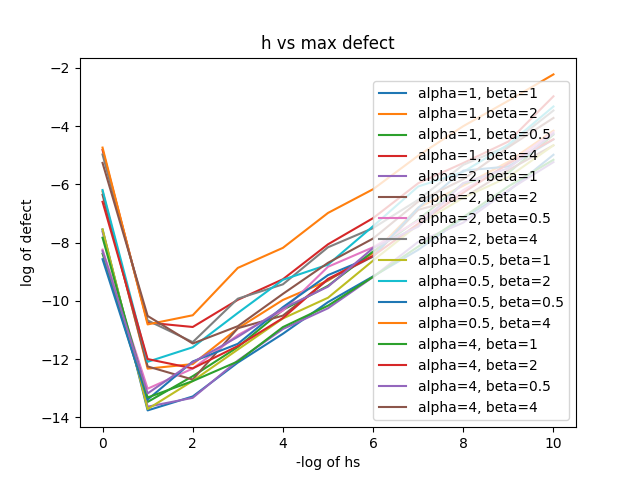
\includegraphics[width=0.7\linewidth]{./figures/hb8_second_scheme_alpha_beta_test}
\caption{HB8 Second Scheme - maximum order of accuracy based on different values of alpha and beta}
\label{fig:hb8_second_scheme_alpha_beta_test}
\end{figure}

From Figure $\ref{fig:hb8_second_scheme_alpha_beta_test}$, we can see how this scheme is better than the first scheme. We can vary $\alpha$ and $\beta$ to 2 and to 1/2 and still get a maximum defect of around $10^{-12}$ and we can even be accurate to $10^{-10}$ at both $\alpha$ and $\beta$ at 4. 

For the remainder of this paper, we will denote this $8^{th}$ order interpolant by HB8. Its derivative has order 7 and any subsequent higher derivative will have one less order.

\paragraph{results}
We will now modify RK4 with the second scheme of HB8 and use the new defect control solver to solve the 3 problems. We will show that we can sample the defect only twice to get the maximum defect and that this scheme is viable to defect control.

======================================================
\paragraph{Problem 1 results}
Figures $\ref{fig:rk4_with_hb8_p1_global_defect}$, $\ref{fig:rk4_with_hb8_p1_global_error}$ and $\ref{fig:rk4_with_hb8_p1_scaled_defects}$ shows the results of using the modification of RK4 with HB8 on Problem 1. We note that an absolute tolerance of $10^{-6}$ is applied on the maximum defect within the step and this can be shown to occur at $0.4h$ and $0.8h$ along a step of size, h. See Figure $\ref{fig:rk4_with_hb8_p1_scaled_defects}$ to see the scaled defect peaking at these points. We note that we successfully control the defect and thus successfully control the error.

\begin{figure}[H]
\centering
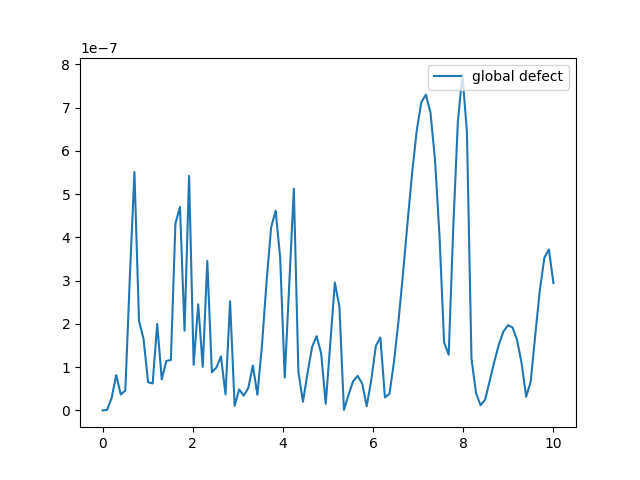
\includegraphics[width=0.7\linewidth]{./figures/rk4_with_hb8_p1_global_defect}
\caption{Global Defect of RK4 with HB8 on problem 1 at an absolute tolerance of $10^{-6}$}
\label{fig:rk4_with_hb8_p1_global_defect}
\end{figure}

\begin{figure}[H]
\centering
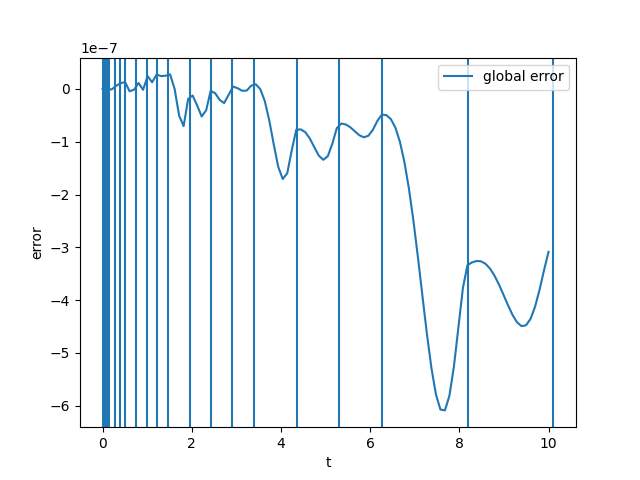
\includegraphics[width=0.7\linewidth]{./figures/rk4_with_hb8_p1_global_error}
\caption{Global Error of RK4 with HB8 on problem 1 at an absolute tolerance of $10^{-6}$}
\label{fig:rk4_with_hb8_p1_global_error}
\end{figure}

\begin{figure}[H]
\centering
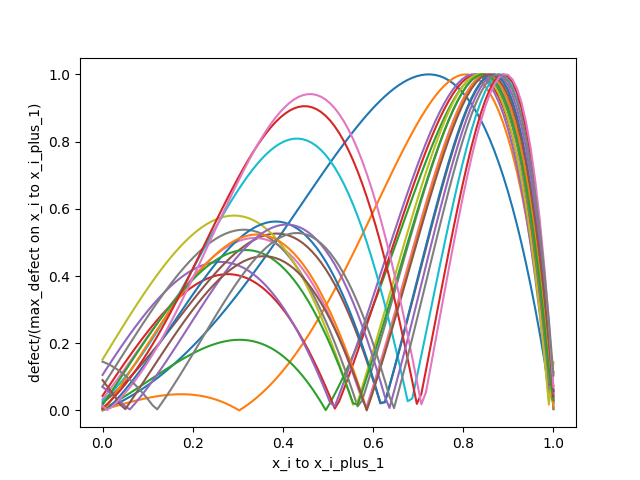
\includegraphics[width=0.7\linewidth]{./figures/rk4_with_hb8_p1_scaled_defects}
\caption{Scaled Defects of RK4 with HB8 on problem 1 at an absolute tolerance of $10^{-6}$}
\label{fig:rk4_with_hb8_p1_scaled_defects}
\end{figure}

\paragraph{Problem 2 results}
Figures $\ref{fig:rk4_with_hb8_p2_global_defect}$, $\ref{fig:rk4_with_hb8_p2_global_error}$ and $\ref{fig:rk4_with_hb8_p2_scaled_defects}$ shows the results of using the modification of RK4 with HB6 on Problem 2. We note that an absolute tolerance of $10^{-6}$ is applied on the maximum defect within the step and this can be shown to occur at $0.8h$ along a step of size, h. See Figure $\ref{fig:rk4_with_hb8_p2_scaled_defects}$ to see the scaled defect peeking at these points. We note that we successfully control the defect and thus successfully control the error.

\begin{figure}[H]
\centering
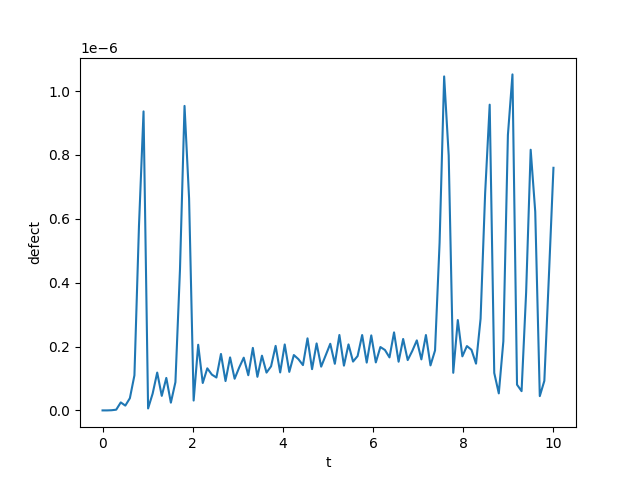
\includegraphics[width=0.7\linewidth]{./figures/rk4_with_hb8_p2_global_defect}
\caption{Global Defect of RK4 with HB8 on problem 2 at an absolute tolerance of $10^{-6}$}
\label{fig:rk4_with_hb8_p2_global_defect}
\end{figure}

\begin{figure}[H]
\centering
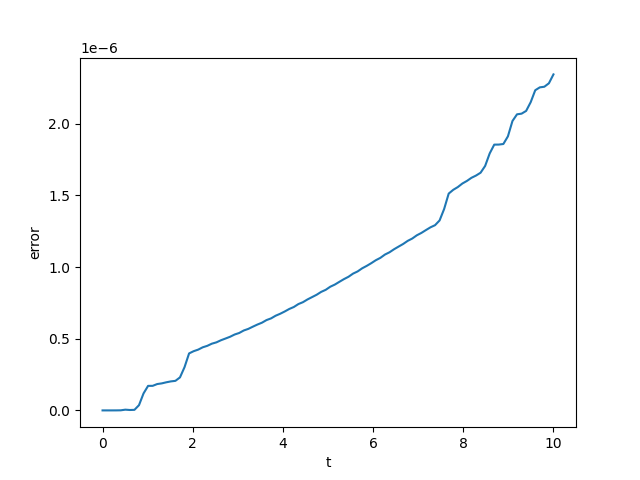
\includegraphics[width=0.7\linewidth]{./figures/rk4_with_hb8_p2_global_error}
\caption{Global Error of RK4 with HB8 on problem 2 at an absolute tolerance of $10^{-6}$}
\label{fig:rk4_with_hb8_p2_global_error}
\end{figure}

\begin{figure}[H]
\centering
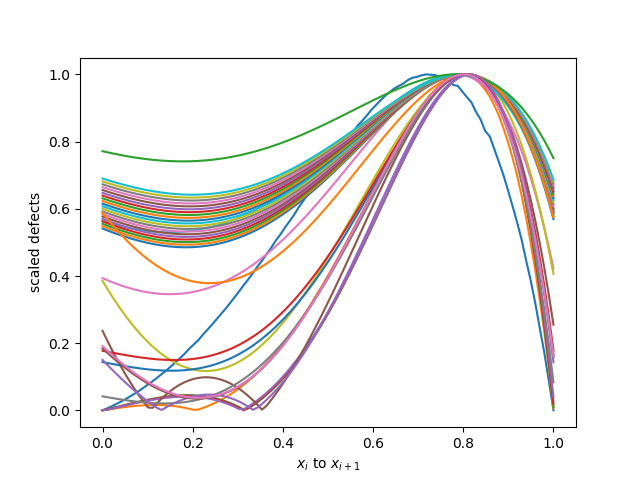
\includegraphics[width=0.7\linewidth]{./figures/rk4_with_hb8_p2_scaled_defects}
\caption{Scaled Defects of RK4 with HB8 on problem 2 at an absolute tolerance of $10^{-6}$}
\label{fig:rk4_with_hb8_p2_scaled_defects}
\end{figure}

\paragraph{Problem 3 results}
Figures $\ref{fig:rk4_with_hb8_p3_global_defect}$, $\ref{fig:rk4_with_hb8_p3_global_error}$ and $\ref{fig:rk4_with_hb8_p3_scaled_defects}$ shows the results of using the modification of RK4 with HB6 on Problem 3. 
We note that an absolute tolerance of $10^{-6}$ is applied on the maximum defect within the step and this can be shown to occur at $0.8h$ along a step of size, h. See Figure $\ref{fig:rk4_with_hb8_p3_scaled_defects}$ to see the scaled defect peeking at these points. We note that we successfully control the defect and thus successfully control the error.

\begin{figure}[H]
\centering
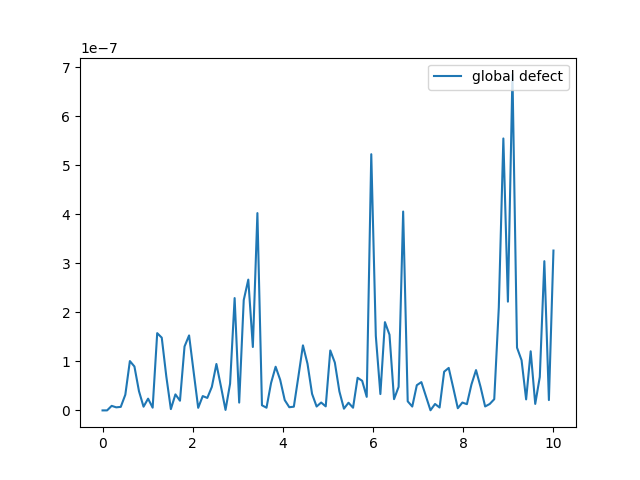
\includegraphics[width=0.7\linewidth]{./figures/rk4_with_hb8_p3_global_defect}
\caption{Global Defect of RK4 with HB8 on problem 3 at an absolute tolerance of $10^{-6}$}
\label{fig:rk4_with_hb8_p3_global_defect}
\end{figure}

\begin{figure}[H]
\centering
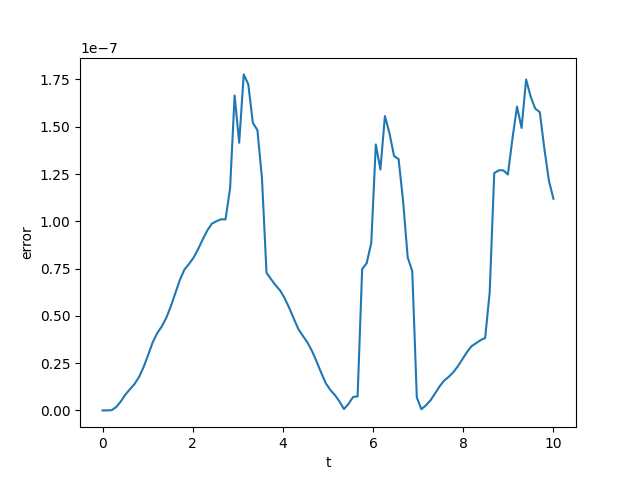
\includegraphics[width=0.7\linewidth]{./figures/rk4_with_hb8_p3_global_error}
\caption{Global Error of RK4 with HB8 on problem 3 at an absolute tolerance of $10^{-6}$}
\label{fig:rk4_with_hb8_p3_global_error}
\end{figure}

\begin{figure}[H]
\centering
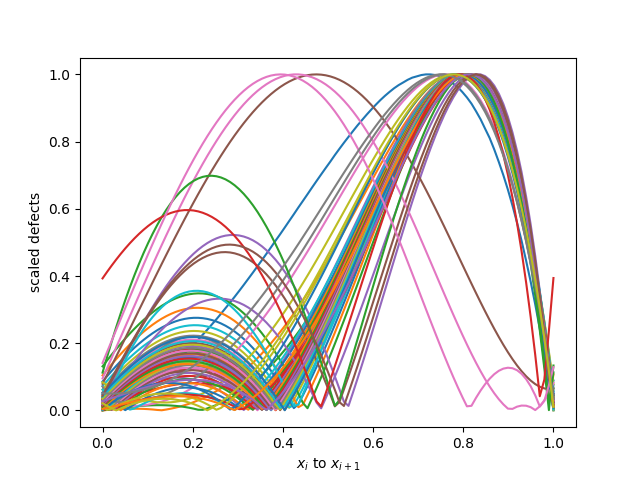
\includegraphics[width=0.7\linewidth]{./figures/rk4_with_hb8_p3_scaled_defects}
\caption{Scaled Defects of RK4 with HB8 on problem 3 at an absolute tolerance of $10^{-6}$}
\label{fig:rk4_with_hb8_p3_scaled_defects}
\end{figure}

We note that the defects are not as clean they were in the case with HB4. There are two peaks most of the time at around $0.4h$ and $0.8h$ but as was the case in the third problem, the peak sometimes comes at $0.6h$. However, we can see that the defect is still being controlled and thus that the error is still being controlled. We will also see that it is twice as fast as it uses around half the number of steps as HB4.

\begin{table}[h]
\caption {Number of steps taken by RK4 when modified to do defect control with HB8 vs when modified with HB6} \label{tab:rk4_with_hb8_nsteps}
\begin{center}
\begin{tabular}{ c c c c c } 
Problem & n. successful steps HB8 & n. successful steps HB6 & nsteps HB8 & nsteps HB6 \\ 
1       & 18                      &        26               & 18         & 31\\ 
2       & 41                      &        36               & 74         & 66\\
3       & 72                      &        63               & 130        & 101\\
\end{tabular}
\end{center}
\end{table}

From Table $\ref{tab:rk4_with_hb8_nsteps}$, we can see that the number of steps with HB6 and with HB8 are relatively similar. This indicates that the interpolation error is no longer the limiting factor, even in HB6. The limiting factor is the ODE solution which is as required. Thus though we can modify RK4 with HB8 at the same cost as modifying RK4 with HB6, using HB8 does not improve the efficiency. Furthermore, HB8 is less stable to changes in $\alpha$ and $\beta$ than HB6 is to changes to $\alpha$. Thus rk4 is best augmented with HB6. However HB8 provides a new opportunity, we can now augment a $6^{th}$ order Runge Kutta method and possibly an $8^{th}$ order Runge-Kutta method, but the interpolation error will still affect it. Augmenting higher order methods with our HB6 and HB8 scheme is a big deal because as we have discussed in Section $\ref{section:crk_related_work}$, the number of stages grows exponentially with the order of the method in the previous works. Our scheme is zero-cost and thus effective defect control will be furthermore impressive.


\subsection{Higher Order Runge Kuttas}
In this section, we attempt to perform defect control on higher order Runge-Kutta methods. We recall that related previous work used significantly more stages to transform a respective $6^{th}$ order discrete Runge-Kutta method to a continuous $6^{th}$ order Runge-Kutta method and same with an $8^{th}$ order Runge-Kutta method.

In this section, we will first augment an rk6 method (See Section $\ref{section:basic_runge_kutta}$ for details about the discrete method) with HB6 and then with HB8. We hope to perform defect control and to replicate that the use of HB8 allows significantly less steps. We will then augment an rk8 method (See Section $\ref{section:basic_runge_kutta}$ for more details) with HB8 to show that though interpolation error is present, the scheme does allow defect control and thus a continuous $8^{th}$ order solution. 

For both method, we will sample the defect only twice in a step, at $0.4h$ and $0.8h$ in a step of size $h$ as the previous experiments seems to indicate that the maximum defect tend to occur at these spots.

\subsubsection{rk6 with HB6}
======================================================
\paragraph{Problem 1 results}
Figures $\ref{fig:rk6_with_hb6_p1_global_defect}$, $\ref{fig:rk6_with_hb6_p1_global_error}$ and $\ref{fig:rk6_with_hb6_p1_scaled_defects}$ shows the results of using the modification of RK6 with HB6 on Problem 1. We note that an absolute tolerance of $10^{-6}$ is applied on the maximum defect within the step and this can be shown to occur at $0.4h$ and $0.8h$ along a step of size, h. See Figure $\ref{fig:rk6_with_hb6_p1_scaled_defects}$ to see the scaled defect peaking at these points. We note that we successfully control the defect and thus successfully control the error.

\begin{figure}[H]
\centering
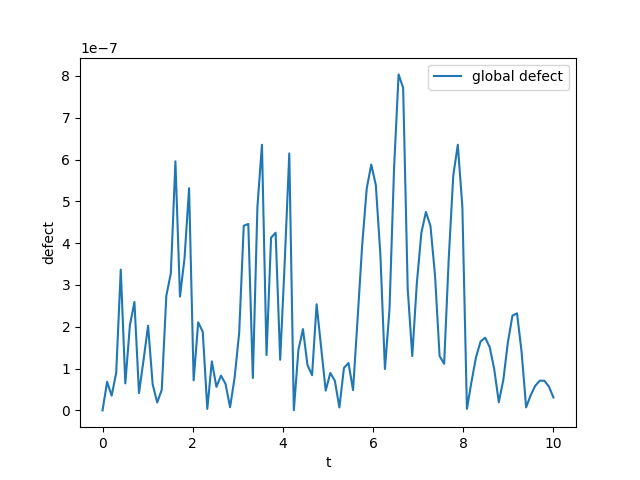
\includegraphics[width=0.7\linewidth]{./figures/rk6_with_hb6_p1_global_defect}
\caption{Global Defect of RK6 with HB6 on problem 1 at an absolute tolerance of $10^{-6}$}
\label{fig:rk6_with_hb6_p1_global_defect}
\end{figure}

\begin{figure}[H]
\centering
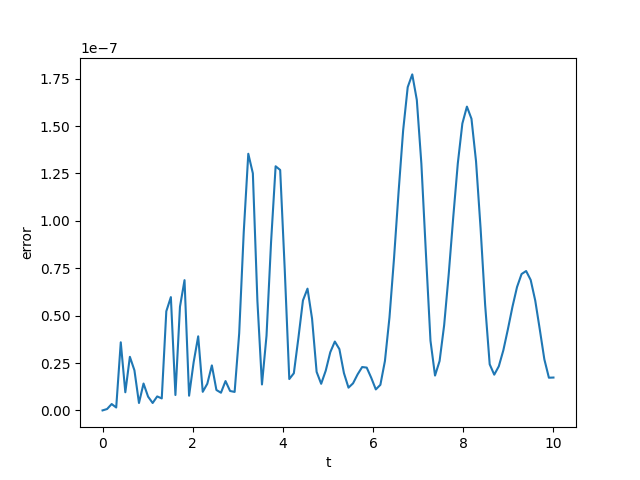
\includegraphics[width=0.7\linewidth]{./figures/rk6_with_hb6_p1_global_error}
\caption{Global Error of RK6 with HB6 on problem 1 at an absolute tolerance of $10^{-6}$}
\label{fig:rk6_with_hb6_p1_global_error}
\end{figure}

\begin{figure}[H]
\centering
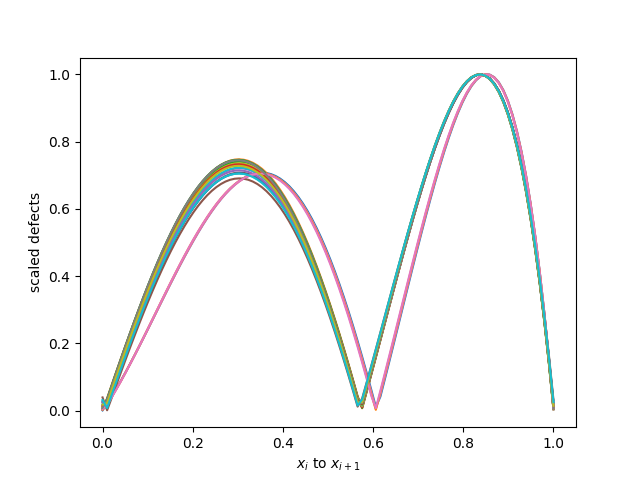
\includegraphics[width=0.7\linewidth]{./figures/rk6_with_hb6_p1_scaled_defects}
\caption{Scaled Defects of RK6 with HB6 on problem 1 at an absolute tolerance of $10^{-6}$}
\label{fig:rk6_with_hb6_p1_scaled_defects}
\end{figure}

\paragraph{Problem 2 results}
Figures $\ref{fig:rk6_with_hb6_p2_global_defect}$, $\ref{fig:rk6_with_hb6_p2_global_error}$ and $\ref{fig:rk6_with_hb6_p2_scaled_defects}$ shows the results of using the modification of RK6 with HB6 on Problem 2. We note that an absolute tolerance of $10^{-6}$ is applied on the maximum defect within the step and this can be shown to occur at $0.8h$ along a step of size, h. See Figure $\ref{fig:rk6_with_hb6_p2_scaled_defects}$ to see the scaled defect peeking at these points. We note that we successfully control the defect and thus successfully control the error.

\begin{figure}[H]
\centering
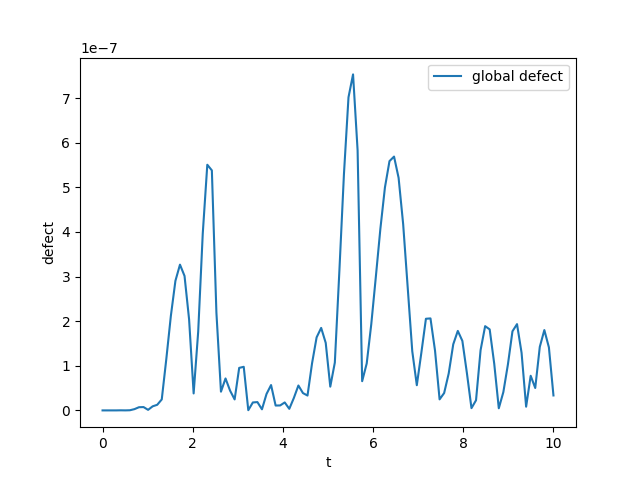
\includegraphics[width=0.7\linewidth]{./figures/rk6_with_hb6_p2_global_defect}
\caption{Global Defect of RK6 with HB6 on problem 2 at an absolute tolerance of $10^{-6}$}
\label{fig:rk6_with_hb6_p2_global_defect}
\end{figure}

\begin{figure}[H]
\centering
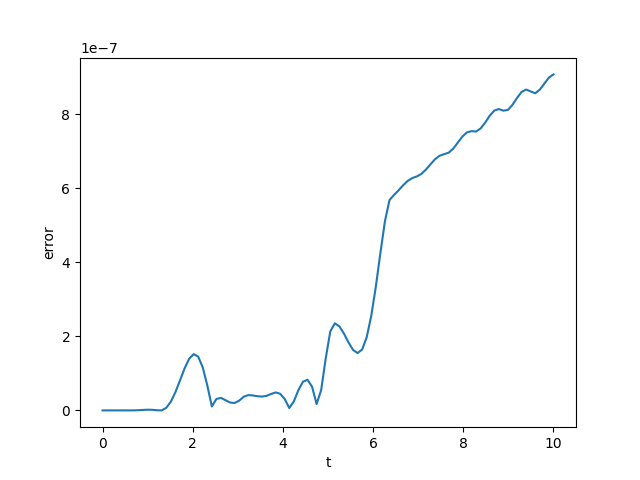
\includegraphics[width=0.7\linewidth]{./figures/rk6_with_hb6_p2_global_error}
\caption{Global Error of RK6 with HB6 on problem 2 at an absolute tolerance of $10^{-6}$}
\label{fig:rk6_with_hb6_p2_global_error}
\end{figure}

\begin{figure}[H]
\centering
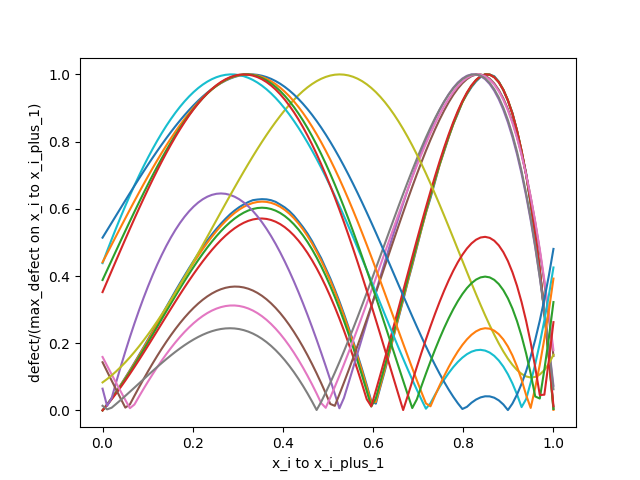
\includegraphics[width=0.7\linewidth]{./figures/rk6_with_hb6_p2_scaled_defects}
\caption{Scaled Defects of RK6 with HB6 on problem 2 at an absolute tolerance of $10^{-6}$}
\label{fig:rk6_with_hb6_p2_scaled_defects}
\end{figure}

\begin{figure}[H]
\centering
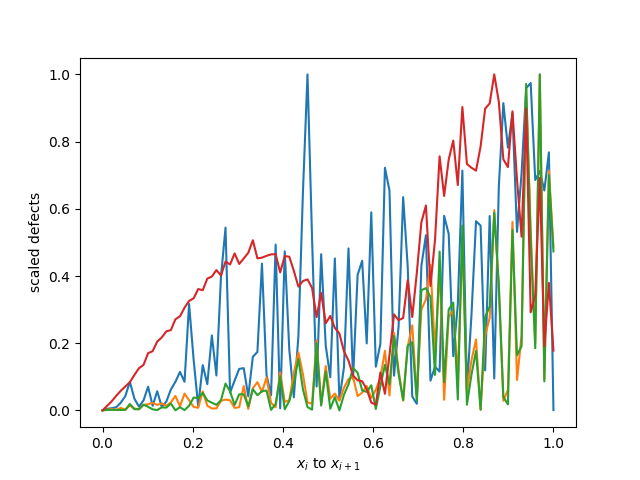
\includegraphics[width=0.7\linewidth]{./figures/rk6_with_hb6_p2_scaled_defects_small_steps}
\caption{Scaled Defects of RK6 with HB6 on small steps on problem 2 at an absolute tolerance of $10^{-6}$}
\label{fig:rk6_with_hb6_p2_scaled_defects_small_steps}
\end{figure}

\paragraph{Problem 3 results}
Figures $\ref{fig:rk6_with_hb6_p3_global_defect}$, $\ref{fig:rk6_with_hb6_p3_global_error}$ and $\ref{fig:rk6_with_hb6_p3_scaled_defects}$ shows the results of using the modification of RK6 with HB6 on Problem 3. 
We note that an absolute tolerance of $10^{-6}$ is applied on the maximum defect within the step and this can be shown to occur at $0.8h$ along a step of size, h. See Figure $\ref{fig:rk6_with_hb6_p3_scaled_defects}$ to see the scaled defect peeking at these points. We note that we successfully control the defect and thus successfully control the error.

\begin{figure}[H]
\centering
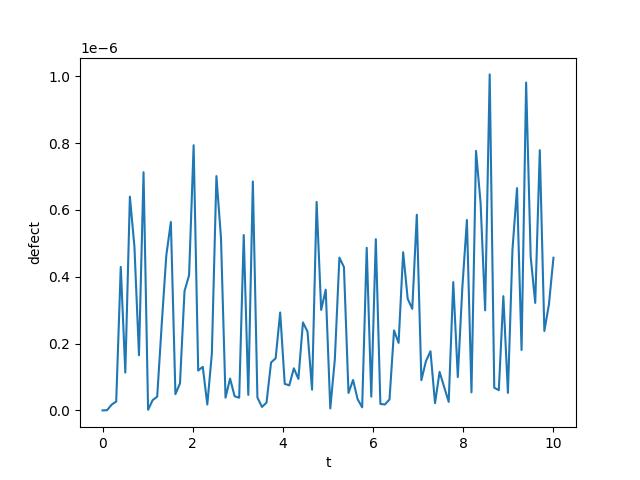
\includegraphics[width=0.7\linewidth]{./figures/rk6_with_hb6_p3_global_defect}
\caption{Global Defect of RK6 with HB6 on problem 3 at an absolute tolerance of $10^{-6}$}
\label{fig:rk6_with_hb6_p3_global_defect}
\end{figure}

\begin{figure}[H]
\centering
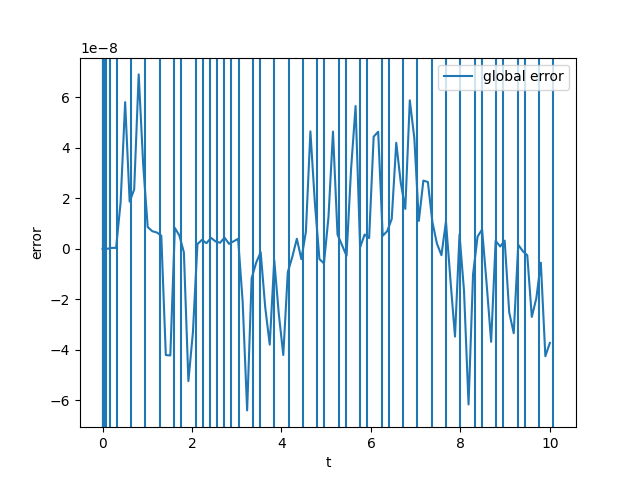
\includegraphics[width=0.7\linewidth]{./figures/rk6_with_hb6_p3_global_error}
\caption{Global Error of RK6 with HB6 on problem 3 at an absolute tolerance of $10^{-6}$}
\label{fig:rk6_with_hb6_p3_global_error}
\end{figure}

\begin{figure}[H]
\centering
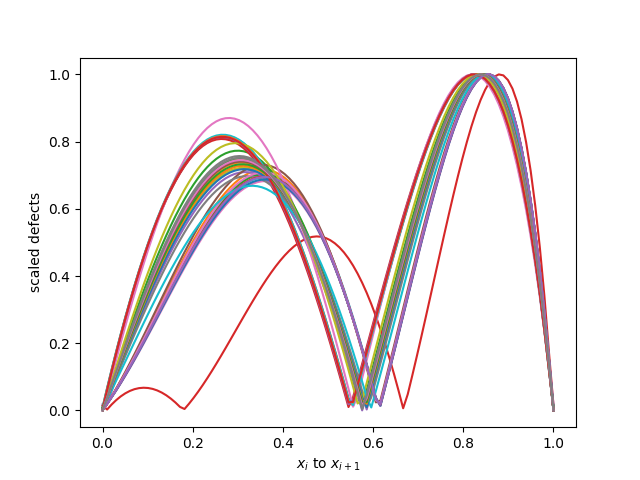
\includegraphics[width=0.7\linewidth]{./figures/rk6_with_hb6_p3_scaled_defects}
\caption{Scaled Defects of RK6 with HB6 on problem 3 at an absolute tolerance of $10^{-6}$}
\label{fig:rk6_with_hb6_p3_scaled_defects}
\end{figure}

\begin{figure}[H]
\centering
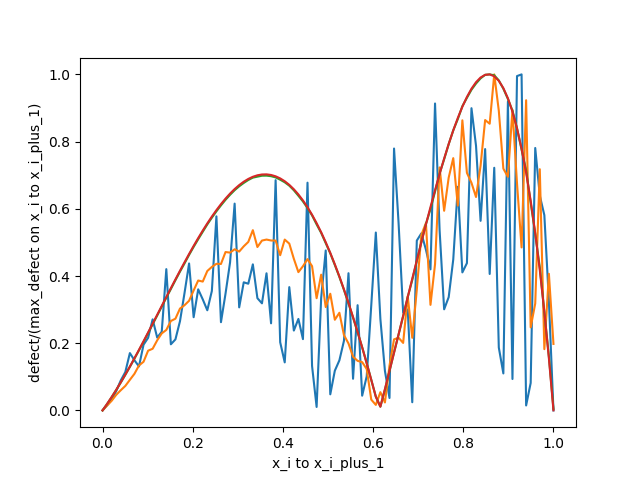
\includegraphics[width=0.7\linewidth]{./figures/rk6_with_hb6_p3_scaled_defects_small_steps}
\caption{Scaled Defects of RK6 with HB6 on small steps on problem 3 at an absolute tolerance of $10^{-6}$}
\label{fig:rk6_with_hb6_p3_scaled_defects_small_steps}
\end{figure}

======================================

\subsubsection{rk6 with HB8}
======================================================
\paragraph{Problem 1 results}
Figures $\ref{fig:rk6_with_hb8_p1_global_defect}$, $\ref{fig:rk6_with_hb8_p1_global_error}$ and $\ref{fig:rk6_with_hb8_p1_scaled_defects}$ shows the results of using the modification of RK6 with HB8 on Problem 1. We note that an absolute tolerance of $10^{-6}$ is applied on the maximum defect within the step and this can be shown to occur at $0.4h$ and $0.8h$ along a step of size, h. See Figure $\ref{fig:rk6_with_hb8_p1_scaled_defects}$ to see the scaled defect peaking at these points. We note that we successfully control the defect and thus successfully control the error.

\begin{figure}[H]
\centering
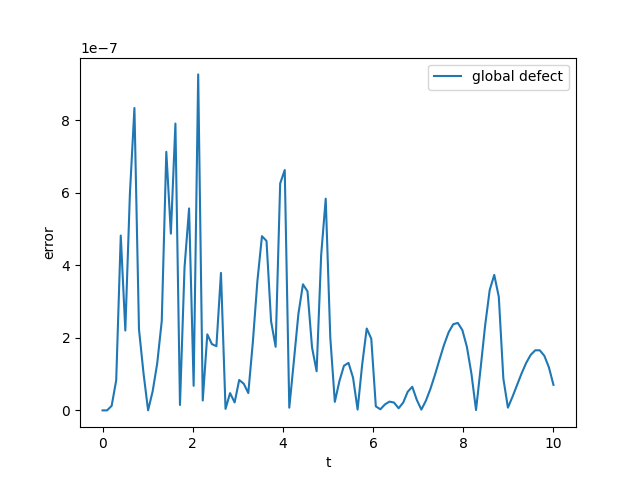
\includegraphics[width=0.7\linewidth]{./figures/rk6_with_hb8_p1_global_defect}
\caption{Global Defect of RK6 with HB8 on problem 1 at an absolute tolerance of $10^{-6}$}
\label{fig:rk6_with_hb8_p1_global_defect}
\end{figure}

\begin{figure}[H]
\centering
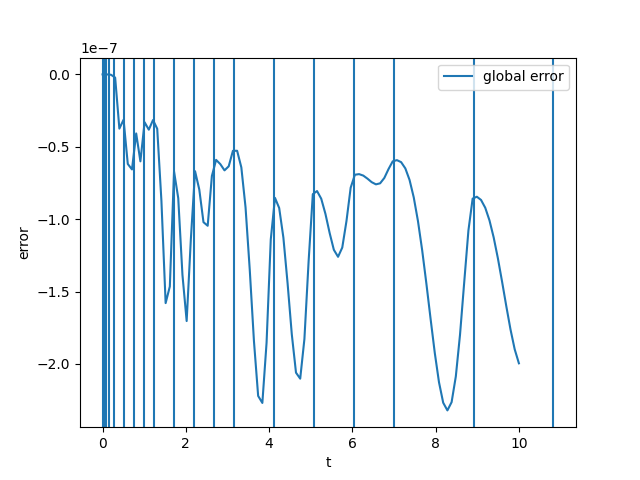
\includegraphics[width=0.7\linewidth]{./figures/rk6_with_hb8_p1_global_error}
\caption{Global Error of RK6 with HB8 on problem 1 at an absolute tolerance of $10^{-6}$}
\label{fig:rk6_with_hb8_p1_global_error}
\end{figure}

\begin{figure}[H]
\centering
\includegraphics[width=0.7\linewidth]{./figures/rk6_with_hb8_p1_scaled_defects}
\caption{Scaled Defects of RK6 with HB8 on problem 1 at an absolute tolerance of $10^{-6}$}
\label{fig:rk6_with_hb8_p1_scaled_defects}
\end{figure}

\paragraph{Problem 2 results}
Figures $\ref{fig:rk6_with_hb8_p2_global_defect}$, $\ref{fig:rk6_with_hb8_p2_global_error}$ and $\ref{fig:rk6_with_hb8_p2_scaled_defects}$ shows the results of using the modification of RK6 with HB8 on Problem 2. We note that an absolute tolerance of $10^{-6}$ is applied on the maximum defect within the step and this can be shown to occur at $0.8h$ along a step of size, h. See Figure $\ref{fig:rk6_with_hb8_p2_scaled_defects}$ to see the scaled defect peeking at these points. We note that we successfully control the defect and thus successfully control the error.

\begin{figure}[H]
\centering
\includegraphics[width=0.7\linewidth]{./figures/rk6_with_hb8_p2_global_defect}
\caption{Global Defect of RK6 with HB8 on problem 2 at an absolute tolerance of $10^{-6}$}
\label{fig:rk6_with_hb8_p2_global_defect}
\end{figure}

\begin{figure}[H]
\centering
\includegraphics[width=0.7\linewidth]{./figures/rk6_with_hb8_p2_global_error}
\caption{Global Error of RK6 with HB8 on problem 2 at an absolute tolerance of $10^{-6}$}
\label{fig:rk6_with_hb8_p2_global_error}
\end{figure}

\begin{figure}[H]
\centering
\includegraphics[width=0.7\linewidth]{./figures/rk6_with_hb8_p2_scaled_defects}
\caption{Scaled Defects of RK6 with HB8 on problem 2 at an absolute tolerance of $10^{-6}$}
\label{fig:rk6_with_hb8_p2_scaled_defects}
\end{figure}

\begin{figure}[H]
\centering
\includegraphics[width=0.7\linewidth]{./figures/rk6_with_hb8_p2_scaled_defects_small_steps}
\caption{Scaled Defects of RK6 with HB8 on small steps on problem 2 at an absolute tolerance of $10^{-6}$}
\label{fig:rk6_with_hb8_p2_scaled_defects_small_steps}
\end{figure}

\paragraph{Problem 3 results}
Figures $\ref{fig:rk6_with_hb8_p3_global_defect}$, $\ref{fig:rk6_with_hb8_p3_global_error}$ and $\ref{fig:rk6_with_hb8_p3_scaled_defects}$ shows the results of using the modification of RK6 with HB8 on Problem 3. 
We note that an absolute tolerance of $10^{-6}$ is applied on the maximum defect within the step and this can be shown to occur at $0.8h$ along a step of size, h. See Figure $\ref{fig:rk6_with_hb8_p3_scaled_defects}$ to see the scaled defect peeking at these points. We note that we successfully control the defect and thus successfully control the error.

\begin{figure}[H]
\centering
\includegraphics[width=0.7\linewidth]{./figures/rk6_with_hb8_p3_global_defect}
\caption{Global Defect of RK6 with HB8 on problem 3 at an absolute tolerance of $10^{-6}$}
\label{fig:rk6_with_hb8_p3_global_defect}
\end{figure}

\begin{figure}[H]
\centering
\includegraphics[width=0.7\linewidth]{./figures/rk6_with_hb8_p3_global_error}
\caption{Global Error of RK6 with HB8 on problem 3 at an absolute tolerance of $10^{-6}$}
\label{fig:rk6_with_hb8_p3_global_error}
\end{figure}

\begin{figure}[H]
\centering
\includegraphics[width=0.7\linewidth]{./figures/rk6_with_hb8_p3_scaled_defects}
\caption{Scaled Defects of RK6 with HB8 on problem 3 at an absolute tolerance of $10^{-6}$}
\label{fig:rk6_with_hb8_p3_scaled_defects}
\end{figure}

\begin{figure}[H]
\centering
\includegraphics[width=0.7\linewidth]{./figures/rk6_with_hb8_p3_scaled_defects_small_steps}
\caption{Scaled Defects of RK6 with HB8 on small steps on problem 3 at an absolute tolerance of $10^{-6}$}
\label{fig:rk6_with_hb8_p3_scaled_defects_small_steps}
\end{figure}

\begin{table}[h]
\caption {Number of steps taken by RK6 when modified to do defect control with HB8 vs when modified with HB6} \label{tab:rk6_with_hb6_vs_hb8_nsteps}
\begin{center}
\begin{tabular}{ c c c c c } 
Problem & n. successful steps HB8 & n. successful steps HB6 & nsteps HB8 & nsteps HB6 \\ 
1       & 17                      &        26               & 18         & 32\\ 
2       & 14                      &        18               & 19         & 26\\
3       & 24                      &        43               & 28         & 61\\
\end{tabular}
\end{center}
\end{table}

From Table $\ref{tab:rk6_with_hb6_vs_hb8_nsteps}$, we can see that again, using an interpolant whose interpolation error and especially interpolation error of its derivative is of higher order than the ODE solution drastically reduces the number of steps. The code becomes more efficient as a result. Since rk6 with HB6 and with HB8 is behaving similarly to rk4 with HB4 and with HB6, we expect that using a $10^{th}$ order method would not improve the situation more than HB8 has over HB6. Though fitting rk6 with HB10 will be as costless as fitting it with HB8, the fact that the interpolation error is no longer the limiting factor means that HB10 will not improve the situation. For rk6, Hb8 is the preferred interpolant.  

We also note that during the solving of the 3 problems, the value of $\alpha$ with HB6 rarely was bigger than 4 or smaller than $\frac{1}{4}$. The values of $\alpha$ and $\beta$ with HB8 also rarely were bigger than 4 or smaller than $\frac{1}{4}$. 

\subsubsection{rk8 with HB8}
In this section, we fit the RK8 method, described in Section $\ref{section:basic_runge_kutta}$, with HB8. Though we expect the interpolation error to reduce the efficiency of this modification, we provide a proof of concept that an RK8 can have defect control with the scheme presented in this chapter. 
===============
We will look into an HB10 scheme later. Depending on time, I may do it as well.
==================
\paragraph{Problem 1 results}
Figures $\ref{fig:rk8_with_hb8_p1_global_defect}$, $\ref{fig:rk8_with_hb8_p1_global_error}$ and $\ref{fig:rk8_with_hb8_p1_scaled_defects}$ shows the results of using the modification of RK8 with HB8 on Problem 1. We note that an absolute tolerance of $10^{-6}$ is applied on the maximum defect within the step and this can be shown to occur at $0.4h$ and $0.8h$ along a step of size, h. See Figure $\ref{fig:rk8_with_hb8_p1_scaled_defects}$ to see the scaled defect peaking at these points. We note that we successfully control the defect and thus successfully control the error.

\begin{figure}[H]
\centering
\includegraphics[width=0.7\linewidth]{./figures/rk8_with_hb8_p1_global_defect}
\caption{Global Defect of RK8 with HB8 on problem 1 at an absolute tolerance of $10^{-6}$}
\label{fig:rk8_with_hb8_p1_global_defect}
\end{figure}

\begin{figure}[H]
\centering
\includegraphics[width=0.7\linewidth]{./figures/rk8_with_hb8_p1_global_error}
\caption{Global Error of RK8 with HB8 on problem 1 at an absolute tolerance of $10^{-6}$}
\label{fig:rk8_with_hb8_p1_global_error}
\end{figure}

\begin{figure}[H]
\centering
\includegraphics[width=0.7\linewidth]{./figures/rk8_with_hb8_p1_scaled_defects}
\caption{Scaled Defects of RK8 with HB8 on problem 1 at an absolute tolerance of $10^{-6}$}
\label{fig:rk8_with_hb8_p1_scaled_defects}
\end{figure}

\paragraph{Problem 2 results}
Figures $\ref{fig:rk8_with_hb8_p2_global_defect}$, $\ref{fig:rk8_with_hb8_p2_global_error}$ and $\ref{fig:rk8_with_hb8_p2_scaled_defects}$ shows the results of using the modification of RK8 with HB8 on Problem 2. We note that an absolute tolerance of $10^{-6}$ is applied on the maximum defect within the step and this can be shown to occur at $0.8h$ along a step of size, h. See Figure $\ref{fig:rk8_with_hb8_p2_scaled_defects}$ to see the scaled defect peeking at these points. We note that we successfully control the defect and thus successfully control the error.

\begin{figure}[H]
\centering
\includegraphics[width=0.7\linewidth]{./figures/rk8_with_hb8_p2_global_defect}
\caption{Global Defect of RK8 with HB8 on problem 2 at an absolute tolerance of $10^{-6}$}
\label{fig:rk8_with_hb8_p2_global_defect}
\end{figure}

\begin{figure}[H]
\centering
\includegraphics[width=0.7\linewidth]{./figures/rk8_with_hb8_p2_global_error}
\caption{Global Error of RK8 with HB8 on problem 2 at an absolute tolerance of $10^{-6}$}
\label{fig:rk8_with_hb8_p2_global_error}
\end{figure}

\begin{figure}[H]
\centering
\includegraphics[width=0.7\linewidth]{./figures/rk8_with_hb8_p2_scaled_defects}
\caption{Scaled Defects of RK8 with HB8 on problem 2 at an absolute tolerance of $10^{-6}$}
\label{fig:rk8_with_hb8_p2_scaled_defects}
\end{figure}

\begin{figure}[H]
\centering
\includegraphics[width=0.7\linewidth]{./figures/rk8_with_hb8_p2_scaled_defects_small_steps}
\caption{Scaled Defects of RK8 with HB8 on small steps on problem 2 at an absolute tolerance of $10^{-6}$}
\label{fig:rk8_with_hb8_p2_scaled_defects_small_steps}
\end{figure}

\paragraph{Problem 3 results}
Figures $\ref{fig:rk8_with_hb8_p3_global_defect}$, $\ref{fig:rk8_with_hb8_p3_global_error}$ and $\ref{fig:rk8_with_hb8_p3_scaled_defects}$ shows the results of using the modification of RK8 with HB8 on Problem 3. 
We note that an absolute tolerance of $10^{-6}$ is applied on the maximum defect within the step and this can be shown to occur at $0.8h$ along a step of size, h. See Figure $\ref{fig:rk8_with_hb8_p3_scaled_defects}$ to see the scaled defect peeking at these points. We note that we successfully control the defect and thus successfully control the error.

\begin{figure}[H]
\centering
\includegraphics[width=0.7\linewidth]{./figures/rk8_with_hb8_p3_global_defect}
\caption{Global Defect of RK8 with HB8 on problem 3 at an absolute tolerance of $10^{-6}$}
\label{fig:rk8_with_hb8_p3_global_defect}
\end{figure}

\begin{figure}[H]
\centering
\includegraphics[width=0.7\linewidth]{./figures/rk8_with_hb8_p3_global_error}
\caption{Global Error of RK8 with HB8 on problem 3 at an absolute tolerance of $10^{-6}$}
\label{fig:rk8_with_hb8_p3_global_error}
\end{figure}

\begin{figure}[H]
\centering
\includegraphics[width=0.7\linewidth]{./figures/rk8_with_hb8_p3_scaled_defects}
\caption{Scaled Defects of RK8 with HB8 on problem 3 at an absolute tolerance of $10^{-6}$}
\label{fig:rk8_with_hb8_p3_scaled_defects}
\end{figure}

\begin{figure}[H]
\centering
\includegraphics[width=0.7\linewidth]{./figures/rk8_with_hb8_p3_scaled_defects_small_steps}
\caption{Scaled Defects of RK8 with HB8 on small steps on problem 3 at an absolute tolerance of $10^{-6}$}
\label{fig:rk8_with_hb8_p3_scaled_defects_small_steps}
\end{figure}

\subsection{the Vshaped graph - defect vs error control with HB scheme}
\label{section:v_shaped_graph}

\subsubsection{HB6}
show that several problems with the interpolant run on random data points) have the same optimal h. 
Possibility to derive optimal h. This way a solver based on this approach will try BIG steps. if failed we reduce the step to that optimal h. If failed still, we cannot solve the problem.

\subsubsection{HB8}
show that several problems with the interpolant run on random data points) have the same optimal h. 
Possibility to derive optimal h. This way a solver based on this approach will try BIG steps. if failed we reduce the step to that optimal h. If failed still, we cannot solve the problem.

\subsection{Low cost with alpha = 1, interpolation}
\label{section:keeping_alpha_at_1}
Because we have interpolants on all previous steps. We can use these interpolants to look up:
basically for HB6
	if going from $x_i$ to $x_{i_plus_1}$ with a step of size h.
	we can look up $x_{i_minus_1}$ using alpha=1 with previousInterps.eval($x_i$ - h) for $y_{i_minus_1}$ and previousInterps.prime($x_i$ - h) for $f_{i_minus_1}$
	
Show results of rk4 with hb6 static alpha to show that we can get defect control with that idea.

basically for HB8
		if going from $x_i$ to $x_i{_plus_1}$ with a step of size h.
	we can look up $x_{i_minus_1}$ with previousInterps.eval($x_i$ - h) for $y_{i_minus_1}$ and previousInterps.prime($x_i$ - h) for $f_{i_minus_1}$
	we can look up $x_{i_minus_2}$ with previousInterps.eval($x_{i_minus_1}$ - h) for $y_{i_minus_2}$ and previousInterps.prime($x_{i_minus_1}$ - h) for $f_{i_minus_2}$.
	
show results of rk4 with hb8 static alpha to show that we get defect control
	
\subsubsection{pros}
Some cost to do derivative evals of new solution values

=============
Isn't it no cost => need to talk with professor
===============

\subsubsection{problems}
the first step. we may have to artificially restrict the GROWTH in the step-size.
for example:
if we go from t0 to t0 + h and the error estimate is much lower than the tolerance, we cannot use a step size of 2*h as t0 + h - 2*h = t0-h but we dont have an interpolant in the region < t0.

\subsection{Solving at high tolerances}

\subsection{Future work}
\subsubsection{additional problems to solve to get this to work}
\paragraph{the first/first and second step}
take an error control step with a stricter tolerance than the user provided tolerance. 
Take a CRK interpolant step.

\paragraph{V-shaped error}
Derive optimal h. keep solver using BIG steps. reduce to optimal h.

\paragraph{static alpha}
use variable alpha for the first few steps. Usually not a problem as in all our experiments alpha is at a good values.
If alpha goes to 8, use static alpha.

\paragraph{noisy defect on small step-sizes}
Trial with horner method and Barycentric method.

\end{document}